\section{理论结果}
\label{sec:results}

本节的推导沿两个估计目标、两个误差下限、不可约分量的识别与监测设计依次展开（表~\ref{tab:roadmap}）。瞬时再生数的误差下限随规模趋于零；跨期平均再生数的误差下限含环境方差 $v_R$，报告率逐期波动时再加上报告异质性方差 $v_H$。随后讨论这两个分量能否从计数中分开和估准，最后把结论写成规模、期数与报告口径之间的预算分配。命题~\ref{prop:current}、命题~\ref{prop:average}、注~\ref{rem:reporting}、命题~\ref{prop:allocation} 与第~\ref{sec:res-test}~节的增长检验分别是 Cramér--Rao 不等式、全方差公式、两阶段抽样与单调似然比检验的标准结果，它们提供后文所用的记号与设计量。新的结果是覆盖与报告率排序的反转阈值（推论~\ref{cor:switch}）、截距随滞后权重变化的 $F$ 签名（命题~\ref{prop:report-noise}(vi)）、环境方差估计的有效期数 $T_{\mathrm{eff}}$（命题~\ref{prop:vR-info}(iii)），以及自相关环境下由预算阈值决定的期数与规模设计（命题~\ref{prop:ar-design}）。

\begin{table}[!tbp]
  \centering
  \small
  \caption{第~\ref{sec:results}~节的推导路线与主要符号。(a) 各步处理的问题及对应结果；(b) 符号、含义与首次定义的位置。}
  \label{tab:roadmap}
  \begin{tabular}{@{}lll@{}}
    \toprule
    \multicolumn{3}{@{}l}{(a) 推导路线}\\
    步骤 & 问题 & 结果\\
    \midrule
    估计目标 & 监测关心当期 $R_t$ 还是跨期平均 $\Rbar$ & 第~\ref{sec:meth-targets}~节\\
    下限一 & $R_t$ 的估计误差随规模能降到多低 & 命题~\ref{prop:current}\\
    下限二 & $\Rbar$ 的误差中哪些项不随规模下降 & 命题~\ref{prop:average}、命题~\ref{prop:report-noise}(i)--(iii)\\
    识别 & 不可约分量能否从计数中分开、估准 & 命题~\ref{prop:report-noise}(v)(vi)、命题~\ref{prop:vR-info}、推论~\ref{cor:season}\\
    设计 & 预算如何在规模、期数与报告口径之间分配 & 命题~\ref{prop:allocation}、推论~\ref{cor:switch}、命题~\ref{prop:levers}、命题~\ref{prop:ar-design}\\
    \midrule
    \multicolumn{3}{@{}l}{(b) 主要符号}\\
    符号 & 含义 & 定义位置\\
    \midrule
    $R_t$，$\Rbar$，$v_R$ & 瞬时再生数、跨期平均再生数、环境方差 & 第~\ref{sec:meth-targets}~节\\
    $n$，$\rho$，$m=\rho n$ & 上一代感染者数、报告率、预计报告规模 & 第~\ref{sec:meth-model}~节\\
    $k$ & 继发感染数的负二项离散参数 & 式~\eqref{eq:offspring}\\
    $A$，$\mx=A/v_R$ & 规模项系数、方差平衡规模 & 式~\eqref{eq:var-average}\\
    $p_t$，$\tau$，$v_H$，$A_H$ & 随机报告率、其相对波动、报告异质性方差及规模项系数 & H5、式~\eqref{eq:r3-vH}\\
    $\phi$，$\psi$ & $R_t$ 与报告冲击的一阶自相关系数 & 第~\ref{sec:res-average}、\ref{sec:r3-reporting}~节\\
    $T$，$c_0$，$c_1$，$\mathcal B$ & 期数、每期固定成本、每例边际成本、总预算 & 命题~\ref{prop:allocation}\\
    $w$，$F(w,\psi)$，$q_j$，$r_j$ & 滞后权重、截距签名函数、截距比、斜率比 & 式~\eqref{eq:r3-F}，第~\ref{sec:meth-renewal}~节\\
    \bottomrule
  \end{tabular}
\end{table}

\subsection{瞬时再生数的估计精度}
\label{sec:res-current}

瞬时再生数能被测到多准，由单期报告数关于 $R_t$ 的 Fisher 信息决定。对估计目标1，$R_t$ 视为固定参数，估计量的性质由式~\eqref{eq:report-dist} 直接决定。

\begin{proposition}[瞬时再生数的有效估计]
\label{prop:current}
在 H1--H3 下，给定 $n$ 与 $R_t>0$，估计量 $\widehat R_t=C_t/m$ 满足：
\begin{enumerate}[label=(\roman*)]
  \item $\widehat R_t$ 是 $R_t$ 的极大似然估计；当 $C_t=0$ 时，似然在边界 $R_t=0$ 处取最大值；
  \item $\widehat R_t$ 无偏，方差为 $\Var(\widehat R_t\mid n,R_t)=R_t/(\rho n)+R_t^2/(kn)$；
  \item 对任意 $n$，该方差都等于 Cramér--Rao 下界 $1/\mathcal I(R_t)$，其中 $\mathcal I(R_t)=n/(R_t/\rho+{R_t}^2/k)$；
  \item $\widehat R_t$ 是 $R_t$ 的一致最小方差无偏估计。
\end{enumerate}
\end{proposition}

结论 (i)--(iii) 由得分函数得到（证明见补充材料 S1.1 节），(iii) 在每个有限 $n$ 处成立，并非渐近结果。结论 (iv) 来自单参数指数族中 $C_t$ 的完备充分性，要求 $k$ 已知\citep{lehmann1998point, casella2002statistical}。方差的两部分与式~\eqref{eq:relvar} 的两项一一对应，$R_t/(\rho n)$ 来自报告抽样，$R_t^2/(kn)$ 来自超传播；两部分都按 $1/n$ 衰减。Fisher 信息可改写为 $\mathcal I(R_t)=(m/R_t)(1+\rho R_t/k)^{-1}$，$k\to\infty$ 时趋于 $m/R_t$，与 Parag 等\citep{parag2022quantifying}在泊松更新模型下给出的发病曲线信息一致（感染压力取 $n$，报告比例取 $\rho$）。超传播使每个预计报告病例所含的信息按因子 $(1+\rho R_t/k)^{-1}$ 缩减。蒙特卡洛模拟在 $m$ 从 1 到 1000 的 10 个规模上各重复 20,000 次，模拟方差与下界之比为 0.98--1.02（图~\ref{fig:variance}a 空心圆）。只要监测关心的是当期传播强度，扩大规模的收益就不会饱和。

\subsection{跨期平均再生数的误差与环境方差}
\label{sec:res-average}

监测目标换成各期再生数所围绕的跨期平均 $\Rbar$ 以后，误差中有一部分不再随规模下降，其大小由环境方差决定。

\begin{proposition}[跨期平均再生数的估计方差]
\label{prop:average}
在 H1--H4 下，$\widehat R_t=C_t/m$ 是 $\Rbar$ 的无偏估计，其方差为：
\begin{equation}
  V(m)=\Var(\widehat R_t\mid n)=v_R+\frac{\Rbar}{\rho n}+\frac{\Rbar^2+v_R}{kn}
  =v_R+\frac{A}{m},\qquad A=\Rbar+\frac{\rho(\Rbar^2+v_R)}{k}.
  \label{eq:var-average}
\end{equation}
定义方差平衡规模 $\mx=A/v_R$，则：
\begin{enumerate}[label=(\roman*)]
  \item $m\to\infty$ 时 $V(m)\to v_R$。
  \item 规模项在总方差中的份额为 $1/(1+m/\mx)$，在 $m=\mx$ 处两项各占一半。
  \item 规模从 $m$ 翻倍到 $2m$，方差下降的比例为 $1/[2(1+m/\mx)]$。
  \item $V(m)$ 严格递减且严格凸，对 $m$ 的弹性为 $-\mx/(m+\mx)$，在 $m=\mx$ 处等于 $-1/2$。
  \item 在对 $R_t$ 条件无偏的估计类中，$V(m)$ 是 $\Rbar$ 的最小均方误差；在 H4 下（要求各期环境独立，即 $\phi=0$），它也是以过去数据预测下一期增长 $C_{t+1}/m$ 的最小预测均方误差。
\end{enumerate}
\end{proposition}

式~\eqref{eq:var-average} 由全方差公式得到，条件方差的期望给出 $A/m$，条件均值 $R_t$ 的方差给出 $v_R$。比较命题~\ref{prop:current} 可知 $A/m=\E[1/\mathcal I(R_t)]$，估计目标2的方差等于环境方差加上估计目标1的 Cramér--Rao 下界在环境分布上的平均。结论 (v) 即式~\eqref{eq:unbiased-bound} 与式~\eqref{eq:predict-bound}。全方差分解是标准工具，由它导出的设计量是方差平衡规模 $\mx$。

$V(m)$ 处处凸，曲线上没有拐点，方差平衡规模给出的是一个量纲为病例数的比较基准。规模低于 $\mx$ 时，误差主要来自病例数不足；规模高于 $\mx$ 时，误差主要来自环境波动，翻倍带来的方差降幅很快变小。图~\ref{fig:variance} 取 $\Rbar=1.15$、$v_R=0.04$、$k=0.35$、$\rho=0.25$，对应 $A=2.1232$，$\mx=53.1$；规模为 10、53.1 和 200 时，翻倍带来的方差降幅依次为 42.1\%、25.0\% 和 10.5\%。估计目标2的模拟方差与式~\eqref{eq:var-average} 之比同样在 0.98--1.02 之间。

\begin{figure}[!tbp]
  \centering
  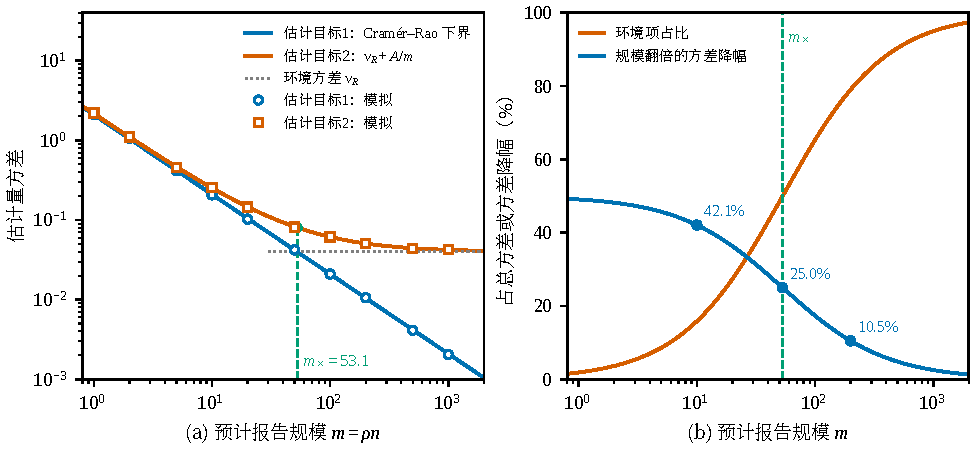
\includegraphics[width=\textwidth]{figures/fig_02_variance_theory.pdf}
  \caption{两个估计目标的方差结构。参数为 $\overline{R}=1.15$，$v_R=0.04$，$k=0.35$，$\rho=0.25$，对应 $A=2.1232$，$m_\times=53.1$。(a) 估计目标1的方差（Cramér--Rao 下界，取 $R_t=\overline{R}$）与估计目标2的方差 $v_R+A/m$ 随预计报告规模的变化；空心点为每个规模 20,000 次模拟的方差（10 个规模），绿色虚线标出方差平衡规模，点线为环境方差。(b) 环境项在估计目标2总方差中的占比，以及规模翻倍带来的方差降幅；三个标注点对应 $m=10$、$m_\times$ 与 $200$。}
  \label{fig:variance}
\end{figure}

环境方差 $v_R$ 作为下确界的适用范围由结论 (v) 限定，即单期、对 $R_t$ 条件无偏的估计，以及 $\phi=0$ 时的一步前瞻预测。$R_t$ 服从系数为 $\phi$ 的一阶自回归时，借用前期信息作预测，不可约的环境部分为 $(1-\phi^2)v_R$，$\phi=0.5$ 与 $0.8$ 时分别为 $0.75v_R$ 与 $0.36v_R$。目标换成 $T$ 期平均时，环境项按式~\eqref{eq:ar-sum} 下降；$T=4$、8、26 时，各期独立的情形分别为 $v_R$ 的 0.250、0.125、0.038 倍，$\phi=0.8$ 时为 0.774、0.605、0.287 倍。允许条件偏差的收缩估计也能低于 $v_R$（补充材料 S1.11 节）。

汇总多个辖区同样可以压低环境项。设 $J$ 个辖区的环境方差同为 $v_R$，两两相关系数的平均值为 $\bar c$，等权汇总后的环境项为：
\begin{equation}
  v_R\,\bar c+\frac{v_R(1-\bar c)}{J}.
  \label{eq:pooling}
\end{equation}
各辖区的扰动不完全同步时（$\bar c<1$），汇总能降低环境项；完全同步时汇总无效。

\begin{remark}[报告率与覆盖面]
\label{rem:reporting}
预计报告规模 $m=\rho n$ 可以靠提高报告率 $\rho$ 或扩大覆盖人群 $n$ 增大。在 H1--H4 下，固定 $n$ 令 $\rho\to1$ 时 $V\to v_R+\Rbar/n+(\Rbar^2+v_R)/(kn)$，极限严格大于 $v_R$；固定 $\rho$ 令 $n\to\infty$ 时 $V\to v_R$。把 $n$ 与 $\rho$ 各提高相同的小比例，前者带来的方差下降是后者的 $A/\Rbar=1+\rho(\Rbar^2+v_R)/(k\Rbar)$ 倍。
\end{remark}

报告完全时超传播项依然存在，只有扩大覆盖才能把方差压到 $v_R$。在图~\ref{fig:variance} 的参数下 $A/\Rbar=1.85$；流感住院占感染的比例约为 0.0056--0.021\citep{zhou2012hospitalizations, tokars2018seasonal}，在第~\ref{sec:res-early}~节的情景参数下该倍数只有 1.02--1.18，两条途径的效果几乎相同，选择主要取决于成本。注~\ref{rem:reporting} 假设报告率在各期固定，报告率随期波动时的排序见推论~\ref{cor:switch}。规模达到 $\mx$ 的量级以后，继续压低趋势估计的误差要靠规模以外的投入。

\subsection{多期分配、成本与增长检验}
\label{sec:res-allocation}
\label{sec:res-test}

总病例量固定时，切成多少期、每期多大，决定了环境项与规模项各自剩下多少。设共观测 $T$ 期，每期预计报告 $m$ 例，总量 $B=Tm$，以各期估计的平均值 $T^{-1}\sum_t\widehat R_t$ 估计 $\Rbar$；每期固定成本为 $c_0$，每例预计报告病例的边际成本为 $c_1$，总经费为 $\mathcal B$，则 $T=\mathcal B/(c_0+c_1m)$。

\begin{proposition}[多期分配与成本]
\label{prop:allocation}
在 H1--H4 下：
\begin{enumerate}[label=(\roman*)]
  \item 若各期 $R_t$ 相互独立，则
  \begin{equation}
    \frac{1}{T^2}\Var({\textstyle\sum_{t=1}^{T}}\widehat R_t)=\frac{v_R}{T}+\frac{A}{B};
    \label{eq:alloc-indep}
  \end{equation}
  若 $R_t$ 服从系数为 $\phi\in(0,1)$ 的平稳一阶自回归，规模项仍为 $A/B$，环境项由式~\eqref{eq:ar-sum} 给出。两种情形下方差都随 $T$ 严格递减。
  \item 独立情形下，计入成本的估计方差为 $f(m)=(c_0+c_1m)(v_R+A/m)/\mathcal B$。$c_0>0$ 时它在
  \begin{equation}
    m^*=\sqrt{\frac{c_0}{c_1}\,\mx},\qquad
    f(m^*)=\frac{(\sqrt{c_0v_R}+\sqrt{c_1A})^2}{\mathcal B}
    \label{eq:optimal-m}
  \end{equation}
  处取最小值；若 $\mathcal B<c_0+c_1m^*$，约束 $T\geq1$ 起作用，最优解取 $T=1$；若 $c_0=0$，最优解为 $m\to0$。
\end{enumerate}
\end{proposition}

总量固定时，规模项 $A/B$ 与切分方式无关，只看方差时期数越多越好；固定成本使期数不能无限增加，最优单期规模是成本比 $c_0/c_1$ 与 $\mx$ 的几何平均。这一优化与两阶段抽样的费用分配同构\citep{cochran1977sampling}，期数对应初级单元数，$v_R$ 对应初级单元间方差，$A$ 对应单元内方差。常用的有效期数近似 $T(1-\phi)/(1+\phi)$ 只保留了式~\eqref{eq:ar-sum} 右端的第一项，总会高估环境项；$\phi=0.8$ 时，$T=26$ 高估 20.5\%，$T=10$ 高估 65.8\%。按第~\ref{sec:res-early}~节的情景参数，$\mx$ 在 21.3--49.2 之间，$c_0/c_1=10$ 时 $m^*$ 为 14.6--22.2，$c_0/c_1=100$ 时为 46.1--70.1。连续解还需取整：取图示参数及 $c_0=100$、$c_1=1$、$\mathcal B=600$，连续解为 $m^*=72.86$，逐个比较整数期数后最优方案为 $T=3$、$m=100$，方差为 0.02041。环境正相关时最优规模偏离 $m^*$ 的方向取决于预算（命题~\ref{prop:ar-design}）。

增长检验处理的是估计目标1层面的判断，即检验 $H_0\colon R_t\leq1$ 对 $H_1\colon R_t>1$。$C_t$ 的分布族关于 $R_t$ 具有单调似然比；令 $c_\alpha$ 为满足 $P_{R_t=1}(C_t\geq c)\leq\alpha$ 的最小整数，在 $C_t\geq c_\alpha$ 时拒绝 $H_0$，第一类错误概率在 $R_t=1$ 处取到上确界 $\alpha^*\leq\alpha$，检验在水平 $\alpha^*$ 下一致最优，加入随机化的 Karlin--Rubin 检验恰好达到水平 $\alpha$\citep{karlin1956theory, lehmann2005testing}。在 $R_t=1+\delta$ 处的功效为
\begin{equation}
  \beta(n,\delta)=1-F_{\NB}(c_\alpha-1;\ nk,\ k/[k+\rho(1+\delta)]).
  \label{eq:power}
\end{equation}
这些性质依赖 $k$ 已知，推导见补充材料 S1.5 节。常用的 Wald 检验把 $(\widehat R_t-1)/\sqrt{V_0}$ 与正态分位数比较，$V_0=1/(\rho n)+1/(kn)$；它的实际水平同样可以由负二项分布函数精确算出，小规模时系统性地超过名义水平（图~\ref{fig:test}a）。$k=0.1$、$m=5$ 时实际水平为 7.81\%；在 $m<40$ 的范围内，$k=0.1$、$0.35$ 和 $1$ 的最大实际水平分别为 8.03\%、8.75\% 和 10.40\%，精确检验在整个网格上的最大水平为 0.049997。功效随 $n$ 呈锯齿状，以 $k=0.35$、$\delta=0.3$ 为例，$n$ 从 400 增加到 699 的过程中功效下降了 82 次，规模要求因此同时给出首次达到 80\% 功效的规模和此后始终保持 80\% 以上的规模（图~\ref{fig:test}b 以后者表示）。在 $\rho=0.25$、$k=0.35$ 下，$\delta=0.15$、$0.3$、$0.5$ 对应的两种上一代感染者人数依次为 2071/2107、568/581、229/235。

\begin{figure}[!tbp]
  \centering
  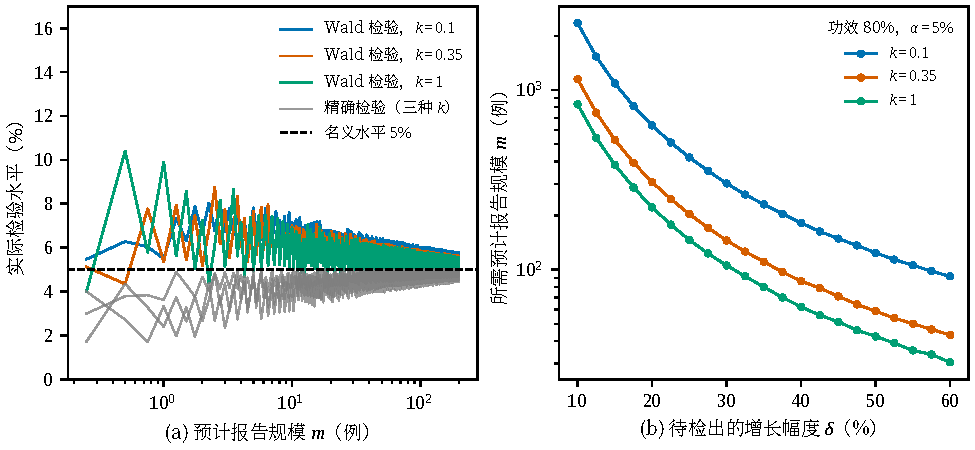
\includegraphics[width=\textwidth]{figures/fig_03_growth_test.pdf}
  \caption{增长检验的实际水平与所需规模，$\rho=0.25$，名义水平 5\%，全部由负二项分布函数精确计算，无模拟误差。(a) Wald 检验（正态近似检验，按 $k$ 着色）与精确检验（灰色）的实际水平随预计报告规模 $m$ 的变化。(b) 达到并保持 80\% 功效所需的预计报告规模与待检出增长幅度 $\delta$ 的关系。}
  \label{fig:test}
\end{figure}

$k=0.35$ 时，稳定检出 15\% 的增长每期需要约 2107 名感染者，即 $m\approx527$，约为图示参数下方差平衡规模的十倍。预警所需的规模应按检验功效单独确定，为趋势估计设定的方差平衡规模在这里并不适用。

\subsection{报告率波动：方差三分量、排序反转阈值与截距的 \texorpdfstring{$F$}{F} 签名}
\label{sec:r3-reporting}

报告比例逐期波动时，不可约误差中多出一个与规模无关的分量，它能否与环境方差在计数中分开需要单独判断。H1 把报告视为固定概率 $\rho$ 的二项抽样，下文用以下假设替代 H1 中的报告部分。

\begin{enumerate}[label=H\arabic*,start=5]
  \item 第 $t$ 期的报告率 $p_t\in(0,1]$ 随机，给定 $p_t$ 时每例新感染独立地以概率 $p_t$ 被报告；$\{p_t\}$ 平稳，与 $\{R_t\}$ 及 $n$ 独立，$\E p_t=\rho$，$\Var p_t=\sigma^2$。记相对波动 $\tau=\sigma/\rho$ 与标准化报告率 $u_t=p_t/\rho$。
  \item 给定 $(R_1,\dots,R_T)$ 与 $(p_1,\dots,p_T)$，各期报告数相互独立。
\end{enumerate}

把式~\eqref{eq:thinning} 推导中的 $\rho$ 换成 $p_t$，即得 $C_t\mid n,R_t,p_t\sim\NB(nk,\,k/(k+p_tR_t))$。二项型波动来自报告率本身的抽样，例如 $p_t\sim\mathrm{Beta}(\rho\nu,(1-\rho)\nu)$，此时 $\sigma^2=\rho(1-\rho)/(\nu+1)$，$\rho\to1$ 时波动消失；制度型波动来自填报口径或检测政策的变化，相对波动 $\tau$ 与 $\rho$ 无关。

\begin{proposition}[报告率波动下的方差三分量]
\label{prop:report-noise}
在 H1--H5 下，记 $U=(1+\tau^2)(\Rbar^2+v_R)$。

\noindent\textsf{分解}
\begin{enumerate}[label=(\roman*)]
  \item 条件方差为：
  \begin{equation}
    \Var(C_t\mid n,R_t)=\rho nR_t+\frac{(\rho^2+\sigma^2)\,nR_t^2}{k}+\sigma^2n^2R_t^2 .
    \label{eq:r3-var-cond}
  \end{equation}
  \item $\widehat R_t=C_t/m$ 仍是 $\Rbar$ 的无偏估计，方差分为三项：
  \begin{equation}
    V_H(m)=v_R+v_H+\frac{A_H}{m},\qquad
    v_H=\tau^2(\Rbar^2+v_R),\qquad
    A_H=\Rbar+\frac{\rho(1+\tau^2)(\Rbar^2+v_R)}{k}.
    \label{eq:r3-vH}
  \end{equation}
  $v_H$ 与覆盖人数 $n$ 无关。推广的方差平衡规模为 $m_{\times,H}=A_H/(v_R+v_H)$。
\end{enumerate}
\noindent\textsf{信息界}
\begin{enumerate}[label=(\roman*),resume]
  \item 记 $\mathcal J_u=\E\{[1+u_tf_u'(u_t)/f_u(u_t)]^2\}$，$f_u$ 为 $u_t$ 的密度。对任一只用 $C_t$ 且对 $R_t$ 条件无偏的估计量 $\tilde\theta$ 与任一规模 $m$，有：
  \begin{equation}
    \E(\tilde\theta-\Rbar)^2\ \geq\ v_R+\frac{\Rbar^2+v_R}{\mathcal J_u},\qquad \mathcal J_u\geq\frac{1}{\tau^2},
    \label{eq:r3-lb}
  \end{equation}
  后一不等式当且仅当 $u_t$ 服从 Gamma 分布时取等号。$u_t$ 服从 Gamma 分布时，下界与规模无关且等于 $v_R+v_H$，$\widehat R_t$ 在 $m\to\infty$ 时趋于该下界，$v_R+v_H$ 因此是这一估计类在全部规模上的下确界。
  \item 若各期报告率 $p_t$ 可观测且 $\E(1/p_t)<\infty$（二项型波动 $p_t\sim\mathrm{Beta}(\rho\nu,(1-\rho)\nu)$ 下即 $\rho\nu>1$，此时 $\E(1/p_t)=(\nu-1)/(\rho\nu-1)$；制度型波动取 $u_t$ 服从 Gamma 分布时即 $\tau<1$），估计量 $\tilde R_t=C_t/(p_tn)$ 对 $R_t$ 条件无偏，均方误差为：
  \begin{equation}
    \E(\tilde R_t-\Rbar)^2=v_R+\frac{\Rbar\,\E(1/p_t)}{n}+\frac{\Rbar^2+v_R}{kn},
    \label{eq:r3-obs}
  \end{equation}
  其中不含 $v_H$；$n\to\infty$ 时趋于 $v_R$。
\end{enumerate}
\noindent\textsf{识别与签名}
\begin{enumerate}[label=(\roman*),resume]
  \item $\E(\widehat R_t)$ 与 $V_H(m)$ 对 $(v_R,\tau^2)$ 的依赖只经过 $U$：$v_R+v_H=U-\Rbar^2$，$A_H=\Rbar+\rho U/k$。只用报告数的前两阶矩，$v_R$ 与 $v_H$ 不可分。
  \item 设第 $j$ 个辖区的报告率为 $p_{j,t}=\rho_ju_{j,t}$，$\rho_j$ 不随时间变化，$u_{j,t}$ 平稳，$\Var u_{j,t}=\tau_w^2$，自相关为 $\psi^h$。增长统计量 $G_t=C_{t+1}/D_t$ 中 $\rho_j$ 精确约去。记 $G_t^0$ 为报告率恒为 $\rho_j$ 时的增长统计量；在无计数噪声、滞后窗口内真实感染数近似不变时，$\E(G_t/G_t^0-1)^2=\tau_w^2F(w,\psi)+o(\tau_w^2)$，其中：
  \begin{equation}
    F(w,\psi)=1-2\sum_{s\geq1}w_s\psi^{s}+\sum_{s\geq1}\sum_{s'\geq1}w_sw_{s'}\psi^{|s-s'|}.
    \label{eq:r3-F}
  \end{equation}
\end{enumerate}
\end{proposition}

\begin{corollary}[覆盖与报告率排序的反转阈值]
\label{cor:switch}
在命题~\ref{prop:report-noise} 的条件下，把 $\rho$ 或 $n$ 各提高相同的小比例，提高报告率带来的方差下降大于扩大覆盖，当且仅当：
\begin{equation}
  -\rho\,\frac{\mathrm d\tau^2}{\mathrm d\rho}\,(kn+1)\ >\ 1+\tau^2 .
  \label{eq:r3-switch}
\end{equation}
二项型波动下，该条件等价于 $m>\rho^2\nu/k$，规模足够大时注~\ref{rem:reporting} 的排序反转；$\nu\to\infty$ 时 $\sigma^2\to0$，条件不再成立。制度型波动下，覆盖与报告率的边际效果之比为 $A_H/\Rbar=1+\rho(1+\tau^2)(\Rbar^2+v_R)/(k\Rbar)>1$，覆盖仍占优，两条途径都不改变 $v_H$。
\end{corollary}

式~\eqref{eq:r3-vH} 在命题~\ref{prop:average} 的两项之外多出 $v_H$，它与环境方差一样不随规模下降。图示参数下取 $\tau=0.15$，$v_H=0.0307$，$A_H=2.145$，推广的方差平衡规模由 53.1 降到 30.4；$m=1000$ 时 $V_H=0.0728$，而 $v_R+A/m=0.0421$。蒙特卡洛在 $\tau\in\{0.15,0.30\}$、$m$ 从 3 到 3000 的 14 个格点上与式~\eqref{eq:r3-vH} 的标准化偏差均小于 1.7。$v_H$ 中没有超传播带来的 $1/k$ 因子，原因是超传播项随 $n$ 下降，报告率波动作用在整期报告数上。结论 (iii) 用数据处理不等式给出规模无法消除的部分：$C_t$ 只经过 $p_tR_t$ 依赖 $R_t$，其 Fisher 信息不超过与 $m$ 无关的 $\mathcal J_u/R_t^2$。$\tau=0.3$ 的 Gamma 波动下，$m=10$、100、1000 时 $C_t$ 的信息为 2.98、7.11、8.25，趋近上界 8.40；对数正态波动下 $(\Rbar^2+v_R)/\mathcal J_u$ 与 $v_H$ 之比为 $\log(1+\tau^2)/\tau^2$，$\tau=0.15$ 时为 0.989。结论 (iv) 的可积条件比 Parag 等\citep{parag2022quantifying}的信息量刻画更强，后者只依赖报告率的几何均值，对任意 Beta 参数都有限，而这里的均方误差依赖 $\E(1/p_t)$。

推论~\ref{cor:switch} 限定了注~\ref{rem:reporting} 的适用范围。二项型波动下，提高报告率还能压低报告率本身的波动，$\rho=0.25$、$k=0.35$、$\nu=100$ 时排序在 $m>17.9$ 处反转，$\nu=1000$ 时在 $m>178.6$ 处反转。制度型波动下，图示参数与 $\tau=0.15$ 给出的边际效果之比为 1.87，与固定报告率时的 1.85 接近，两条途径都留下 $v_H$。去掉 $v_H$ 需要统一报告口径使 $\tau\to0$，或像结论 (iv) 那样把各期报告率纳入估计。结论 (ii)(iii) 刻画报告率未知时波动留下的不可约部分 $v_H$，结论 (iv) 说明报告率可观测时这一部分可以去除。

结论 (v) 说明仅凭病例计数无法区分环境波动与报告波动，截距超出环境方差情景值的部分可以同样好地由 $v_H$ 解释。结论 (vi) 给出辅助检验的依据：辖区之间报告率的固定差异在比值中约去，只有周间波动进入截距，其幅度按 $F(w,\psi)$ 随滞后权重变化。主规格 $w=(0.65,0.25,0.10)$ 下，$\psi=0$ 时 $F=1.495$，$\psi=0.9$ 时 $F=0.217$。平稳条件下纯报告噪声在 $\psi\in[0,1)$ 上给出的截距比为 $q_1\in[0.883,1.338]$、$q_2\in[0.892,1.374]$，上确界在 $\psi\to1$ 时取到；增长期中这一范围扩大，截距比因此要与增长期零假设一起判读（第~\ref{sec:res-inflation}~节）。

全方差分解与 Cramér--Rao 不等式是标准工具\citep{casella2002statistical}，Zamir\citep{zamir1998proof}给出了 Fisher 信息的数据处理不等式，尺度族 Fisher 信息在 Gamma 分布处达到方差约束下的最小值也是已知结果\citep{lehmann1998point}。报告率在州层面恒定时在比值中约去，与 Gostic 等\citep{gostic2020practical}和 Azmon 等\citep{azmon2014estimating}关于恒定漏报不影响再生数估计的结论一致。在此基础上，三分量分解、推论~\ref{cor:switch} 的反转阈值、经由 $U$ 的不可识别性与 $F$ 签名是针对本文观测链导出的。监测系统若要压低 $v_H$，扩大规模与提高报告率都不够，需要统一填报口径或记录各期报告率。

\subsection{环境方差的可估性与有效期数 \texorpdfstring{$T_{\mathrm{eff}}$}{T\_eff}}
\label{sec:r3-vR}

环境方差决定了规模收益何时变小，它本身也要从有限期数的报告数中估计，其精度受期数还是规模支配需要分开回答。本小节取 $\tau=0$，各期规模同为 $m$。

\begin{proposition}[环境方差的估计精度]
\label{prop:vR-info}
在 H1--H4 与 H6 下，记 $Y_t=C_t/m$，$\sigma_Y^2=v_R+A/m$。
\begin{enumerate}[label=(\roman*)]
  \item 单期报告数的边缘方差为 $\Var(C_t)=m\Rbar+(\rho m/k)(\Rbar^2+v_R)+m^2v_R$。由此得到修正矩估计：
  \begin{equation}
    \hat v_R=\frac{S_C^2\,km-\bar C\,km-\rho\bar C^2}{m^2(km+\rho)}
    =\frac{S_Y^2-\varpi(\bar Y)}{1+\rho/(km)},\qquad \varpi(y)=\frac ym+\frac{\rho y^2}{km},
    \label{eq:r3-vhat}
  \end{equation}
  其中 $\bar C$、$S_C^2$ 为 $T$ 期报告数的样本均值与样本方差（除以 $T-1$），$\bar Y$、$S_Y^2$ 类推。
  \item 各期 $R_t$ 独立同分布时，$T\Var(\hat v_R)\to\Omega(m)$，$\Omega(m)$ 随 $m$ 递减，$m\to\infty$ 时趋于与规模无关的平台 $\Omega_\infty=\E(R_t-\Rbar)^4-v_R^2$；$R_t$ 服从 Gamma 分布时 $\Omega_\infty=v_R^2(2+6v_R/\Rbar^2)$。
  \item $R_t$ 服从系数为 $\phi$ 的平稳高斯一阶自回归、$\Rbar$ 已知时，$m\to\infty$ 下的朴素估计 $T^{-1}\sum_t(R_t-\Rbar)^2$ 的方差为 $2v_R^2\kappa_T(\phi^2)/T$，其中 $\kappa_T(x)=1+2\sum_{h=1}^{T-1}(1-h/T)x^h$。等价的有效期数为：
  \begin{equation}
    T_{\mathrm{eff}}=\frac{T}{\kappa_T(\phi^2)}\ \approx\ T\,\frac{1-\phi^2}{1+\phi^2}.
    \label{eq:r3-teff}
  \end{equation}
\end{enumerate}
\end{proposition}

结论 (ii) 说明扩大单期规模只能把 $\hat v_R$ 的方差压到一个由期数决定的平台。有限 $T$ 的精确方差、$\Omega(m)$ 的 $1/m$ 展开与 Fisher 信息上界见补充材料 S1.7 节；$\Omega(m)$ 的单调性在 $m\in[1,10^5]$ 上经数值核对。图示参数下 $\Omega_\infty=2.18\,v_R^2$，$m=10$、100、1000 时 $\Omega(m)/\Omega_\infty$ 依次为 37.5、2.36、1.11。$\Omega(m)$ 在 $m\to\infty$ 处的一阶展开 $\Omega_\infty+\Omega_1/m$（$\Omega_1/\Omega_\infty=108.6$）只适用于大 $m$：$m=10$ 时一阶式给出 11.9，精确值为 37.5；$m=100$ 时为 2.09 与 2.36。蒙特卡洛覆盖 $m\in\{3,\dots,10^4\}$、$T\in\{3,\dots,100\}$、$\phi\in\{0,0.5,0.8\}$ 共 144 个格点（图~\ref{fig:r3-vR}），$\phi=0$ 的 48 个格点上模拟方差与精确式之比在 0.96 与 1.06 之间。由 Fisher 信息上界得到的相对标准误下界为 $(0.505T)^{-1/2}$，$T=3$、10、50 时分别为 0.81、0.45、0.20，与规模无关。

结论 (iii) 修正了平方序列的有效期数。均值的有效期数近似为 $T(1-\phi)/(1+\phi)$，方差估计的有效期数约为 $T(1-\phi^2)/(1+\phi^2)$，后者更大。$\phi=0.8$、$T=26$ 时，均值的近似有效期数为 2.9，平方序列的精确有效期数为 6.2；$T=100$ 时两者为 11.1 与 22.4。$\Rbar$ 未知时样本方差有向下的偏差，$\E S_R^2=v_R(T-\kappa_T(\phi))/(T-1)$；无论用哪一种估计，精度都只取决于 $T$ 与 $\phi$。

\begin{corollary}[季层面成分]
\label{cor:season}
设 $R_t=\Rbar+\eta_{s(t)}+\omega_t$，$\eta_1,\dots,\eta_S$ 为 $S$ 个流行季的共同成分，独立同分布于 $\mathcal N(0,v_S)$，$\omega_t$ 为季内成分。不论辖区数、每季周数和报告规模多大，$v_S$ 的任一无偏估计的相对标准误不低于 $\sqrt{2/S}$；季均值未知、用样本方差估计时为 $\sqrt{2/(S-1)}$。
\end{corollary}

$S=3$ 时两个下界分别为 0.82 和 1.00，$S=4$ 时为 0.71 和 0.82。若 $v_R$ 含季层面共同成分，这一成分的大小无法由三四个流行季确定，增加州数、周数或报告规模都不改变下界；季内成分仍可由大量州周估计。组间方差的精度受组数限制是方差分量模型的标准结论\citep{searle1992variance, cochran1977sampling}，Bartlett\citep{bartlett1946theoretical}给出了样本自协方差的方差公式；负二项观测链下修正矩估计的平台与平方序列的精确有效期数是本文的推导。认识 $v_R$ 的大小要靠积累观测期，其中的季层面成分要靠积累流行季。

\subsection{设计杠杆与自相关环境下的预算设计}
\label{sec:r3-levers}
\label{sec:r3-design}

规模、期数与报告口径各自作用于均方误差的哪一项，以及环境正相关时预算应偏向少而大的期还是多而小的期，决定了监测投入的先后。

\begin{proposition}[规模、期数与报告标准化的分工]
\label{prop:levers}
在 H1--H6 下，设 $R_t$ 的自相关为 $\gamma_R(h)$，$u_t$ 的自相关为 $\gamma_u(h)$，各期规模同为 $m$。$T$ 期平均 $\bar R_T=T^{-1}\sum_t C_t/m$ 的均方误差为：
\begin{equation}
  \E(\bar R_T-\Rbar)^2=\frac{1}{T^2}\sum_{s=1}^{T}\sum_{t=1}^{T}\Bigl\{v_R\gamma_R(h)+\tau^2\gamma_u(h)\bigl[\Rbar^2+v_R\gamma_R(h)\bigr]\Bigr\}+\frac{A_H}{Tm},\qquad h=|s-t|.
  \label{eq:r3-levers}
\end{equation}
由此：
\begin{enumerate}[label=(\roman*)]
  \item 增大 $m$ 只降低最后一项，均方误差的下限是前两类项之和。
  \item 增大 $T$ 降低环境项，也降低自相关可衰减的报告项；报告偏差持续（$\gamma_u\equiv1$）时，报告项对任何 $T$ 都不低于 $\tau^2\Rbar^2$。
  \item 统一报告口径（$\tau=0$）或在估计中使用观测到的 $p_t$，去掉报告项。
  \item $v_R$ 本身的估计精度只随 $T$ 提高（命题~\ref{prop:vR-info}）。
\end{enumerate}
\end{proposition}

一阶自回归情形的闭式、数值例与证明见补充材料 S1.8 节。在 $T=10$、$m=50$、$\tau=0.15$、$\phi=\psi=0.5$ 的基线上，规模扩大 10 倍对均方误差的改善小于期数增加到 4 倍；报告偏差持续时，增加期数对报告项无效（图~\ref{fig:r3-levers}a）。

相邻流行周的传播条件往往相近，环境正相关时多设一期带来的新信息少于独立情形，期数与规模的取舍随之改变。命题~\ref{prop:allocation}(ii) 只处理独立情形。$R_t$ 服从系数为 $\phi\in(0,1)$ 的平稳一阶自回归时，在预算约束 $T(c_0+c_1m)=\mathcal B$ 下最小化 $f_\phi=[v_R\kappa_T(\phi)+A/m]/T$。把 $T$ 当作连续变量，记 $e(T)=\kappa_T(\phi)/T$，并定义：
\begin{equation}
  g_T(\phi)=-T^2e'(T)=\frac{1+\phi}{1-\phi}-\frac{2\phi}{(1-\phi)^2}\Bigl[\frac{2(1-\phi^T)}{T}+\phi^T\ln\phi\Bigr].
  \label{eq:r3-g}
\end{equation}

\begin{proposition}[一阶自回归下的最优期数与规模]
\label{prop:ar-design}
在 H1--H4 下，设 $R_t$ 为系数 $\phi\in(0,1)$ 的平稳一阶自回归，$c_0,c_1>0$。记独立情形的最优规模 $m_0^*=\sqrt{c_0A/(c_1v_R)}$（式~\eqref{eq:optimal-m}）。
\begin{enumerate}[label=(\roman*)]
  \item $g_T(\phi)$ 关于 $T\geq1$ 严格递增，$g_1(\phi)=[1-4\phi+3\phi^2-2\phi^2\ln\phi]/(1-\phi)^2<1$，$\lim_{T\to\infty}g_T(\phi)=(1+\phi)/(1-\phi)>1$；$e(T)$ 严格凸。
  \item $f_\phi$ 在可行区间上严格凸，最优期数 $T^*$ 唯一且随 $\mathcal B$ 递增，整数最优为 $\lfloor T^*\rfloor$ 或 $\lceil T^*\rceil$，$f_\phi'(1)\geq0$ 时取 $T=1$。内点解满足：
  \begin{equation}
    m^*=\frac{m_0^*}{\sqrt{g_{T^*}(\phi)}} .
    \label{eq:r3-mstar}
  \end{equation}
  \item 记 $T^\dagger(\phi)$ 为 $g_T(\phi)=1$ 的唯一根，$\mathcal B^\dagger=T^\dagger(c_0+c_1m_0^*)$。$\mathcal B<\mathcal B^\dagger$ 时 $m^*>m_0^*$，最优方案是更少、更大的期；$\mathcal B>\mathcal B^\dagger$ 时 $m^*<m_0^*$，最优方案是更多、更小的期；$\mathcal B\to\infty$ 时 $m^*\to m_0^*\sqrt{(1-\phi)/(1+\phi)}$。
\end{enumerate}
\end{proposition}

近似 $m^*\approx m_0^*\sqrt{(1-\phi)/(1+\phi)}$ 只在预算远大于 $\mathcal B^\dagger$ 时成立；预算较小时，正相关使最优方案偏向更少、更大的期。取图示参数与 $c_0/c_1=100$（$m_0^*=72.9$），预算阈值如下：
\begin{center}
  \small
  \begin{tabular}{@{}lcccc@{}}
    \toprule
    $\phi$ & 0.3 & 0.5 & 0.8 & 0.9\\
    \midrule
    $T^\dagger$ & 2.51 & 2.96 & 4.48 & 6.13\\
    $\mathcal B^\dagger$ & 433 & 511 & 775 & 1060\\
    \bottomrule
  \end{tabular}
\end{center}
$\phi=0.8$ 时，$\mathcal B=600$ 的最优解为 $T^*=3.06$、$m^*=96.3$，整数最优为 $T=3$、$m=100$，模拟方差为 0.0403，按近似取 $T=5$、$m=20$ 时为 0.0504；$\mathcal B=2000$ 时 $m^*=36.0$，$\mathcal B=60000$ 时 $m^*=24.5$，接近近似值 24.3（图~\ref{fig:r3-levers}b）。

\begin{remark}[空间汇总]
\label{rem:spatial}
用 $J$ 个辖区代替 $T$ 期，辖区间环境扰动的平均相关为 $\bar c$，预算约束为 $J(c_0+c_1m)=\mathcal B$。由式~\eqref{eq:pooling}，均方误差为 $v_R\bar c+[v_R(1-\bar c)+A/m](c_0+c_1m)/\mathcal B$，最优单辖区规模为 $m^*=\sqrt{c_0A/[c_1v_R(1-\bar c)]}$，随 $\bar c$ 上升。
\end{remark}

独立情形对应两阶段抽样的费用分配\citep{cochran1977sampling}，Hamilton\citep{hamilton1994time}给出了一阶自回归的方差和；相关情形下的精确一阶条件、$g_T$ 的单调性、$e(T)$ 的凸性与预算阈值 $\mathcal B^\dagger$ 由本文导出。预算有限且环境正相关时，应先设少而大的期，预算越过 $\mathcal B^\dagger$ 以后再增加期数；辖区间相关越强，越应在少数辖区加深监测。

\begin{figure}[!tbp]
  \centering
  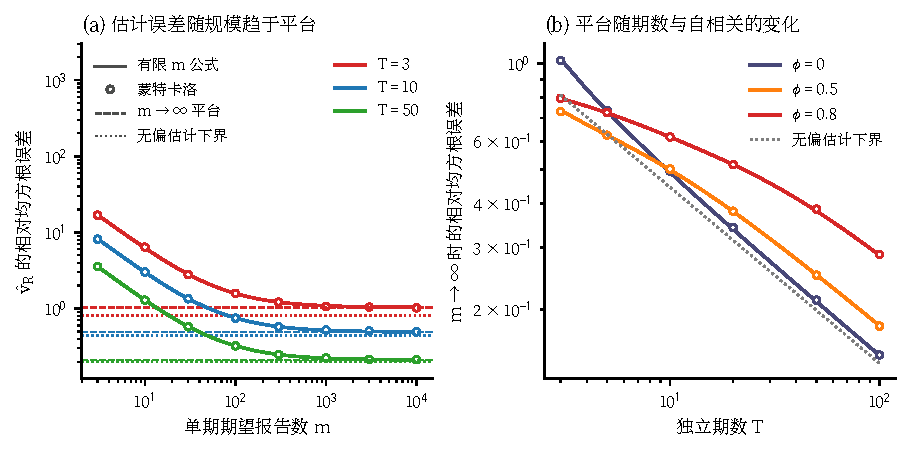
\includegraphics[width=\textwidth]{figures/fig_04_vR_precision.pdf}
  \caption{环境方差估计的精度。参数为 $\overline{R}=1.15$，$v_R=0.04$，$k=0.35$，$\rho=0.25$。(a) 修正矩估计 $\hat v_R$ 的相对均方根误差随单期规模 $m$ 的变化，$R_t$ 独立服从 Gamma 分布；实线为有限规模公式，空心点为每格 20,000 次模拟，虚线为 $m\to\infty$ 的平台，点线为无偏估计的 Fisher 信息下界。(b) $m\to\infty$ 时平台高度随期数 $T$ 的变化；实线为精确值，空心点为 $m=10^4$ 的模拟（$T=100$ 每格 10,000 次，其余 20,000 次）。$\phi=0.8$ 且 $T$ 较小时，均值未知的样本方差有向下的偏差，均方根误差可低于无偏估计下界。}
  \label{fig:r3-vR}
\end{figure}

\begin{figure}[!tbp]
  \centering
  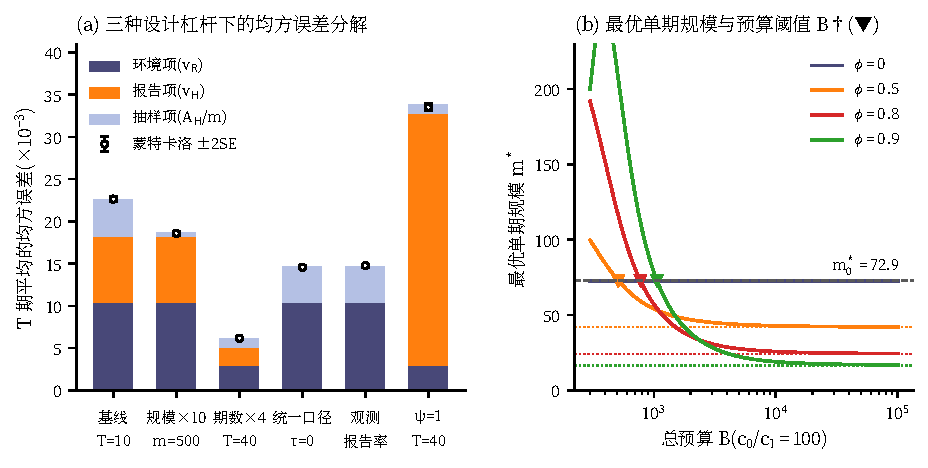
\includegraphics[width=\textwidth]{figures/fig_05_levers_budget.pdf}
  \caption{设计杠杆与预算阈值。(a) $T$ 期平均的均方误差分解，基线为 $T=10$、$m=50$、$\tau=0.15$、$\phi=\psi=0.5$；“规模×10”取 $m=500$，“期数×4”取 $T=40$，“统一口径”取 $\tau=0$，“观测报告率”使用 $C_t/(p_tn)$，“$\psi=1$”为报告偏差在各期持续且 $T=40$。堆叠柱为式~\eqref{eq:r3-levers} 的三类项，空心点为每种设置 60,000 次模拟及其 $\pm2$ 倍标准误。(b) 一阶自回归下最优单期规模随总预算 $\mathcal B$ 的变化，$c_0/c_1=100$；虚线为独立情形的 $m_0^*=72.9$，点线为 $\mathcal B\to\infty$ 的极限 $m_0^*\sqrt{(1-\phi)/(1+\phi)}$，三角标出预算阈值 $\mathcal B^\dagger$。$\phi=0.9$ 的曲线左端位于 $T=1$ 的角点，此时 $m^*=(\mathcal B-c_0)/c_1$ 随预算上升。}
  \label{fig:r3-levers}
\end{figure}

\section{仿真与实证结果}
\label{sec:empirical}

\subsection{更新过程仿真}
\label{sec:res-renewal}

按第~\ref{sec:meth-sim}~节的设置模拟带环境波动的更新过程，结果见图~\ref{fig:renewal}。按初始规模 $m_0$ 计，$m_0\geq25$ 时模拟误差是单代参照曲线的 0.75--0.98 倍。$\Rbar>1$ 使疫情在评价期内增长，实现规模高于初始规模，$D_t/m_0$ 的中位数为 1.86--2.35，误差因而低于按初始规模算出的参照值。按实现规模 $D_t$ 分组，偏离方向相反。$D_t<400$ 时模拟误差是参照的 1.04--1.23 倍，多出的部分来自随机分母；$D_t\geq400$ 时比值为 0.98--1.03，两者基本重合。$m_0$ 很小时误差分布有重尾，$m_0=12$ 时比值为 1.31；$m_0=6$ 时为 2.87，标准误很大，数值不稳定。

\begin{figure}[!tbp]
  \centering
  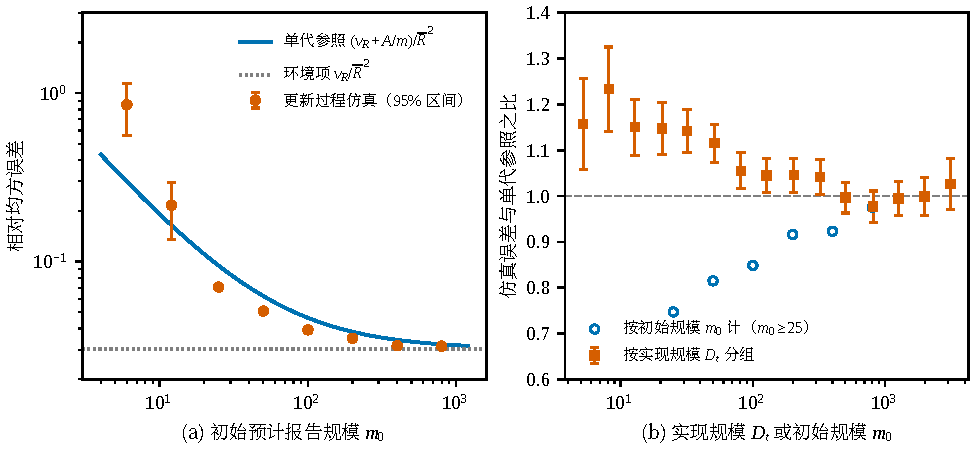
\includegraphics[width=\textwidth]{figures/fig_06_renewal_scale.pdf}
  \caption{更新过程仿真中的规模效应。每个初始规模 400 条轨迹，每条 26 个评价点，误差棒为蒙特卡洛均值 $\pm1.96$ 倍标准误的 95\% 正态近似区间。(a) 增长统计量的相对均方误差随初始预计报告规模 $m_0$ 的变化；实线为单代参照曲线 $(v_R+A/m)/\overline{R}^2$，点线为环境项 $v_R/\overline{R}^2$，参照曲线不构成误差下界。(b) 模拟误差与参照曲线之比，方块按实现规模 $D_t$ 分组，空心圆按初始规模 $m_0$（$m_0\geq25$）计算。}
  \label{fig:renewal}
\end{figure}

参照曲线高估还是低估误差，取决于横轴采用哪种规模。按实现规模计，误差随规模的变化大体保持 $v_R+A/m$ 的形状，小规模处略高。该仿真中各周 $R_t$ 相互独立，$D_t$ 与当期环境无关。$R_t$ 存在时间相关时 H4 不再成立，第~\ref{sec:res-inflation}~节的一阶自回归仿真显示，周间相关系数为 0.5--0.7 时，与规模无关的截距升到独立情形的 1.2--1.4 倍。

\subsection{流感住院数据中误差随规模的变化}
\label{sec:res-early}

实证数据覆盖 50 个州与华盛顿特区，保留 $D_t\geq5$ 的 10,303 个州周（第~\ref{sec:meth-data}~节，图~\ref{fig:nhsn}）。流感的世代间隔约 3 天，一周约跨两代，$G_t$ 的均值和方差都不等于单代再生数的均值和方差。实证分析因此只检验误差随规模变化的形状，拟合系数不作为单代参数的估计。

\begin{figure}[!tbp]
  \centering
  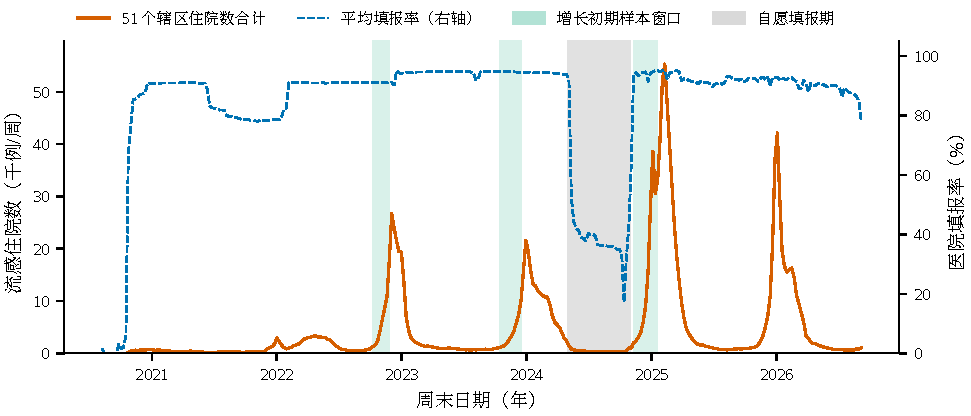
\includegraphics[width=\textwidth]{figures/fig_07_nhsn_series.pdf}
  \caption{美国 51 个辖区每周流感住院数合计（实线，左轴）与医院平均填报率（虚线，右轴）。缺失按 0 计入合计。绿色区间为三个流行季的增长初期样本窗口，灰色区间为 2024 年 5--10 月的自愿填报期。}
  \label{fig:nhsn}
\end{figure}

模型假定各期环境围绕同一均值波动，流行初期最接近这一情形。主分析取三个流行季的增长初期，共 1,267 个州周，平均增长比 $\Rbar_{\mathrm{early}}=1.6706$，标准差 0.7116。误差随规模下降并逐渐趋平（图~\ref{fig:early}）。按 $D_t$ 分为六箱，$[5,20)$ 箱的平均损失为 0.329（$N=319$，95\% 区间 0.244--0.415），$[20,50)$ 箱降到 0.161，$[100,250)$ 箱为 0.112，此后两箱为 0.103 和 0.105。

\begin{figure}[!tbp]
  \centering
  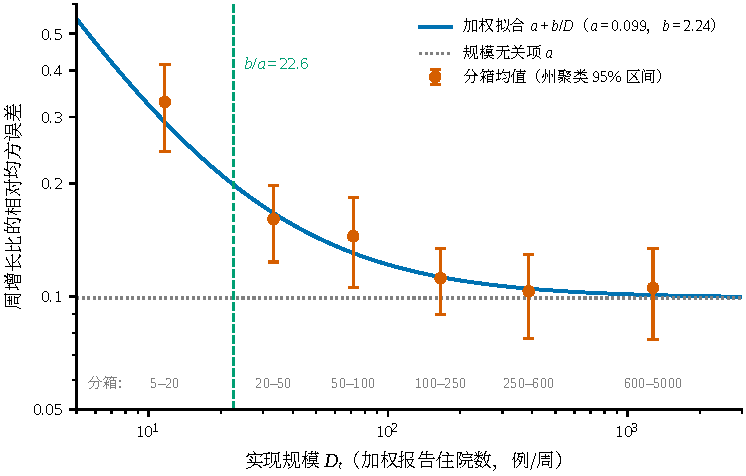
\includegraphics[width=0.8\textwidth]{figures/fig_08_early_scale.pdf}
  \caption{流行初期单步预测误差随实现规模 $D_t$ 的变化，共 1,267 个州周。圆点为各分箱均值，画在箱内平均 $D_t$ 处，误差棒为按州聚类标准误的 95\% 正态近似区间；曲线为 $a+b/D$ 的加权拟合，水平虚线为截距 $a$，竖线为经验比值 $b/a$。}
  \label{fig:early}
\end{figure}

迭代可行广义最小二乘给出 $a=0.0991$（95\% 区间 0.0837--0.1165），$b=2.243$（1.494--3.007），经验比值 $b/a=22.6$ 例/周（13.5--34.9）。BCa 区间分别为 0.0819--0.1144、1.538--3.090 和 14.2--36.6。2,000 次重抽中没有一次 $a\leq0$ 或 $b\leq0$。按州 $\times$ 流行季聚类时，$b$ 的区间为 1.553--2.940。用十分位分组均值拟合同样得到 22.6。损失的离散程度随规模收缩，$\Var(L)/\E(L)^2$ 从最小箱的 5.32 降到最大箱的 0.99，所用权重 $1/\hat\mu^2$ 并非最优；权重只依赖 $D_t$，拟合仍然一致，普通最小二乘给出的 $b=2.305$ 与加权结果接近。

经验比值对极端值敏感。去掉损失最大的 1\% 观测后，$a=0.1077$，$b=1.137$（0.697--1.661），经验比值降到 10.6（5.9--17.3）。改为按周聚类，$b$ 的区间为 1.473--3.119。

误差中存在不随规模消失的部分，这一点得到均值形状比较的支持（表~\ref{tab:shape}）。不含底板的 $L=b/D$ 比仿射形式差得多，留一州交叉验证偏差高 $1949.9\pm243.1$，51 个州中 48 个偏向仿射形式。不含底板的幂律 $L=cD^{-p}$ 给出 $\hat p=0.273$，与仿射形式的偏差差为 $56.8\pm27.2$，约两个标准误，28 个州偏向仿射形式；按未加权平方误差，两者之差为 $3.2\pm3.7$，在一个标准误以内。数据要求误差中含有不随规模消失的部分，但在样本覆盖的规模范围内，不足以区分严格的底板与缓慢的幂律衰减。

\begin{table}[!tbp]
  \centering
  \caption{三种均值形状的比较，主规格流行初期样本（$N=1{,}267$）。各模型用 Gamma 准似然拟合。交叉验证为留一州，基准 $\overline{R}$ 只用训练州估计；差值为相对 M1 的逐州偏差差之和，括号内为州间标准误。}
  \label{tab:shape}
  \small
  \begin{tabular}{@{}llrrrc@{}}
    \toprule
    模型 & 参数估计 & AIC & 交叉验证偏差 & 相对 M1 之差 & 偏向 M1 的州数 \\
    \midrule
    M0：$L=b/D$ & $b=21.7$ & $-1971.2$ & 5407.1 & 1949.9（243.1） & 48/51 \\
    M1：$L=a+b/D$ & $a=0.0991$，$b=2.243$ & $-2718.8$ & 3457.2 & -- & -- \\
    M2：$L=cD^{-p}$ & $c=0.512$，$p=0.273$ & $-2692.6$ & 3514.0 & 56.8（27.2） & 28/51 \\
    \bottomrule
  \end{tabular}
\end{table}


平均损失的分解显示了扩大规模还剩多少空间。样本平均损失为 0.181，其中截距 $a$ 占 54.6\%，规模项 $b/D_t$ 占 45.1\%，拟合残差占 0.2\%，规模项按 $D_t$ 的调和平均数 27.4 计算。作为反事实，把 $D_t<250$ 的州周规模提高到 250、其余州周保持不变，模型给出的平均损失为 0.107，下降 40.9\%。模型在 $D=250$ 处的取值 $a+b/250=0.108$ 是另一个量；实际 $D_t\geq250$ 的 244 个州周平均损失为 0.104，与之接近，但该模型值由拟合机械决定，不构成独立证据。

经验比值与理论情景区间处于同一量级。情景参数取 $\Rbar=1.67$，$k\in[0.2,0.5]$\citep{lloydsmith2005superspreading}，$\rho\in[0.0056,0.021]$\citep{zhou2012hospitalizations, tokars2018seasonal}，$v_R\in[0.04,0.08]$，此时 $A$ 在 1.702--1.971 之间，$\mx$ 在 21.3--49.2 之间。比值吻合不足以检验结构参数。情景隐含的截距为 0.0143--0.0287，斜率为 0.610--0.707；实证 $a$ 是前者的 3.5--6.9 倍，$b$ 是后者的 3.2--3.7 倍。两者被放大的倍数相近，比值才落在情景区间内。下一节用滞后权重的比较考察放大的来源。

\subsection{滞后权重比较与误差机制}
\label{sec:res-inflation}

三种滞后权重为主规格（$\sum w^2=0.495$）、只用当周（$\sum w^2=1$）和三周等权（$\sum w^2=0.333$），实证斜率依次为 2.243、3.134（2.250--4.013）和 1.926（1.083--2.858）。相对主规格，斜率比 $r_1=1.397$（1.229--1.623），$r_2=0.859$（0.599--1.083），区间与基准 $\Rbar$ 在每次重抽中一并重估（表~\ref{tab:ratios}，图~\ref{fig:boot}a,b）。式~\eqref{eq:b-delta} 在情景中点（$\Rbar=1.67$，$v_R=0.06$，$k=0.35$，$\rho=0.021$，$A=1.8409$）的预测为 1.44 和 0.86，全情景网格为 1.419--1.463 和 0.852--0.866，都落在区间内；该情景下三种权重的预测斜率为 1.155、1.660、0.993，情景模拟值为 1.195、1.566、0.999。

斜率比的判别力有限。不含环境方差的 M-bin0 预测 1.432 和 0.862，纯测量误差模型 M-meas 与乘性报告噪声模型 M-mult 预测 1.462 和 0.852，同样落在区间内。区间只排除了分母不含计数噪声的 M-nodn，且只靠 $r_1$。M-nodn 预测两个比值都为 1，1 不在 $r_1$ 的区间内，却在 $r_2$ 的区间内。按州 $\times$ 流行季聚类，两个区间为 1.228--1.617 和 0.633--1.051，结论不变。斜率比说明分母含有报告计数噪声，不能作为环境随机性的证据。

斜率的绝对水平只有一部分能由分母噪声解释。没有分母噪声时，情景斜率为 0.660，约为实证值的 29\%；加入二项噪声后升到 1.155，约为 51\%。报告过程在二项抽样之外的超额离散是剩余部分的一个可能来源，情景模拟中加入这类离散后，模拟斜率可升到 2.019；现有数据无法区分这一来源与其他解释，斜率与截距的绝对水平因此都只得到部分解释。

\begin{table}[!tbp]
  \centering
  \caption{滞后权重比值的实证区间与各误差机制的预测（NHSN 流感流行初期，$N=1{,}267$ 个州周）。$r_1$、$r_2$ 为只用当周、三周等权两种权重相对主规格的斜率比，$q_1$、$q_2$ 为对应的截距比，$a$ 为主规格截距。实证区间为按州聚类 $B=2000$ 次重抽的 95\% 百分位区间，每次重抽都重估 $\overline{R}$。平稳环境模型（M-env）的增长期预测有两种，一种是每周一代的更新仿真（$\phi=0$，9 个情景格子，每格 400 次），另一种是 $\phi=0$ 的日分辨率更新过程。后者取流感世代间隔，环境变异系数平方 CV$^2$ 4 档、世代间隔 3 档、增长率 3 档；不含入院延迟时 36 格，加入无、短、长三档入院延迟后共 108 格，每格 300 次。乘性报告噪声模型（M-mult）的平稳行取报告冲击自相关 $\psi$ 遍历 $[0,1)$ 的解析范围（命题~\ref{prop:report-noise}(vi)）。其增长期行取 $v_R=0$ 与对数一阶自回归报告冲击，$\psi\in\{0,0.3,0.6,0.9\}$、$\tau\in\{0.15,0.3\}$、入院延迟 2 档、增长率 3 档，共 48 格，每格 300 次。其余三类为不含环境方差的二项报告模型（M-bin0）、纯测量误差模型（M-meas）与分母不含计数噪声的模型（M-nodn）。区间型预测为各格模拟平均的最小值至最大值。“--”表示该仿真未计算斜率比，“无截距”表示该机制预测 $a=0$、比值无定义。粗体为与实证区间不相交的预测。}
  \label{tab:ratios}
  \footnotesize
  \setlength{\tabcolsep}{4pt}
  \begin{tabular}{@{}lccccc@{}}
    \toprule
    机制 & $r_1$ & $r_2$ & $q_1$ & $q_2$ & $a$ \\
    \midrule
    实证 & 1.397 & 0.859 & 0.688 & 1.539 & 0.0991 \\
    \quad 95\% 百分位区间 & 1.229--1.623 & 0.599--1.083 & 0.658--0.727 & 1.420--1.656 & 0.0837--0.1165 \\
    \midrule
    M-env，平稳 & 1.419--1.463 & 0.852--0.866 & \textbf{1} & \textbf{1} & $>0$ \\
    M-env，增长期，每周一代 & 1.450--1.630 & 0.693--0.763 & \textbf{0.857--0.937} & \textbf{1.226--1.333} & $>0$ \\
    M-env，增长期，日更新无延迟 & -- & -- & \textbf{0.746--0.887} & 1.319--1.484 & $>0$ \\
    M-env，增长期，日更新全部 & -- & -- & 0.601--0.887 & 1.187--1.568 & $>0$ \\
    M-mult，平稳 & 1.462 & 0.852 & \textbf{0.883--1.338} & \textbf{0.892--1.374} & $>0$ \\
    M-mult，增长期 & -- & -- & 0.686--1.224 & 0.865--1.497 & $>0$ \\
    M-bin0 & 1.432 & 0.862 & 无截距 & 无截距 & \textbf{0} \\
    M-meas & 1.462 & 0.852 & 无截距 & 无截距 & \textbf{0} \\
    M-nodn & \textbf{1.000} & 1.000 & \textbf{1} & \textbf{1} & $>0$ \\
    \bottomrule
  \end{tabular}
\end{table}


截距比的方向在环境各期独立时即可出现，单凭它不能区分机制。实证截距随回溯滞后单调上升，平均滞后为 1.0、1.45、2.0 周时，$a$ 分别为 0.0682（0.0575--0.0815）、0.0991 和 0.1524（0.1271--0.1830）（图~\ref{fig:noise}b）。截距比 $q_1=0.688$（0.658--0.727），$q_2=1.539$（1.420--1.656），2,000 次重抽中 $q_1<1$ 与 $q_2>1$ 的比例都是 100\%（图~\ref{fig:boot}c,d）。平稳环境模型 M-env 与 M-nodn 预测截距与权重无关（$q=1$）；平稳的 M-mult 在报告冲击自相关 $\psi$ 取遍 $[0,1)$ 时可达 $q_1\in[0.883,1.338]$、$q_2\in[0.892,1.374]$（命题~\ref{prop:report-noise}(vi)）；三者都与实证区间不相交。增长期样本改变了这一比较。每周一代的增长期仿真在 $\phi=0$ 下给出 0.857--0.937 与 1.226--1.333，仍在区间外；日分辨率更新过程的 108 个 $\phi=0$ 格子给出 $q_1\in[0.601,0.887]$、$q_2\in[1.187,1.568]$，乘性报告噪声的 48 个增长期格子给出 $[0.686,1.224]$ 与 $[0.865,1.497]$，都与实证区间相交（表~\ref{tab:ratios}）。日分辨率更新过程加入院延迟在 $\phi=0$ 下即可产生 $q_1<1<q_2$ 的截距比特征，故该特征与 $R_t$ 的周间自相关不可区分；本文以截距超出量作为主要证据。扩大零假设范围的主要是入院延迟，不含入院延迟的 36 个日更新格子中 $q_1$ 为 0.746--0.887，仍在实证区间之外。M-bin0 与 M-meas 预测 $a=0$，与截距区间不符，但上一节的幂律比较提示，这一排除依赖仿射形式。情景模拟中三种权重的截距为 0.0225、0.0202、0.0214，几乎不变，分母噪声因而把 $b/a$ 推高到 59.2，而真实的 $A/v_R$ 只有 30.7，用 $b/a$ 估计 $\mx$ 会系统性偏大。三种权重下经验比值在 12.6--46.0 之间变化，它描述的是 $G_t$ 的误差结构，不能作为 $A/v_R$ 的估计。

\begin{figure}[!tbp]
  \centering
  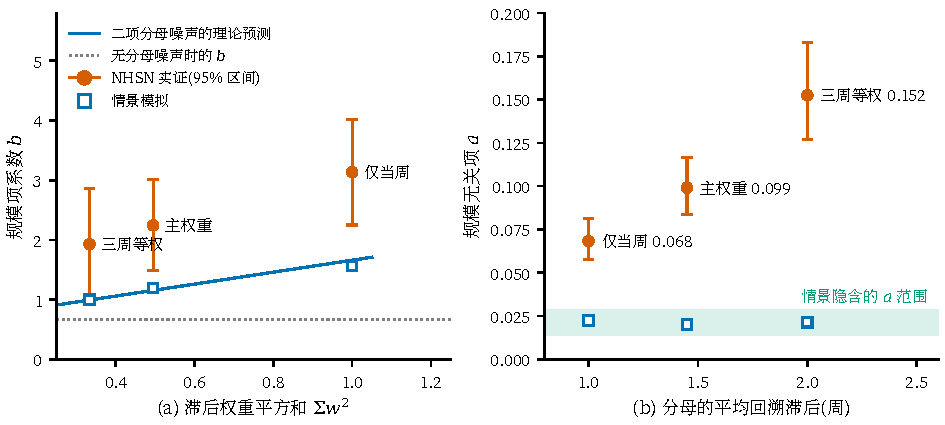
\includegraphics[width=\textwidth]{figures/fig_09_denominator_noise.pdf}
  \caption{滞后权重对拟合系数的影响（NHSN 流感流行初期，$N=1{,}267$ 个州周）。(a) 规模项系数 $b$ 与滞后权重平方和 $\sum w^2$ 的关系。圆点为三种权重的实证估计，误差棒为按州聚类 $B=2000$ 次重抽的 95\% 百分位区间；方块为情景模拟值，实线为二项分母噪声的一阶近似，点线为没有分母噪声时的 $b$。(b) 截距 $a$ 与分母平均回溯滞后的关系，误差棒同 (a)，阴影为情景隐含的截距范围 0.014--0.029。}
  \label{fig:noise}
\end{figure}

\begin{figure}[!tbp]
  \centering
  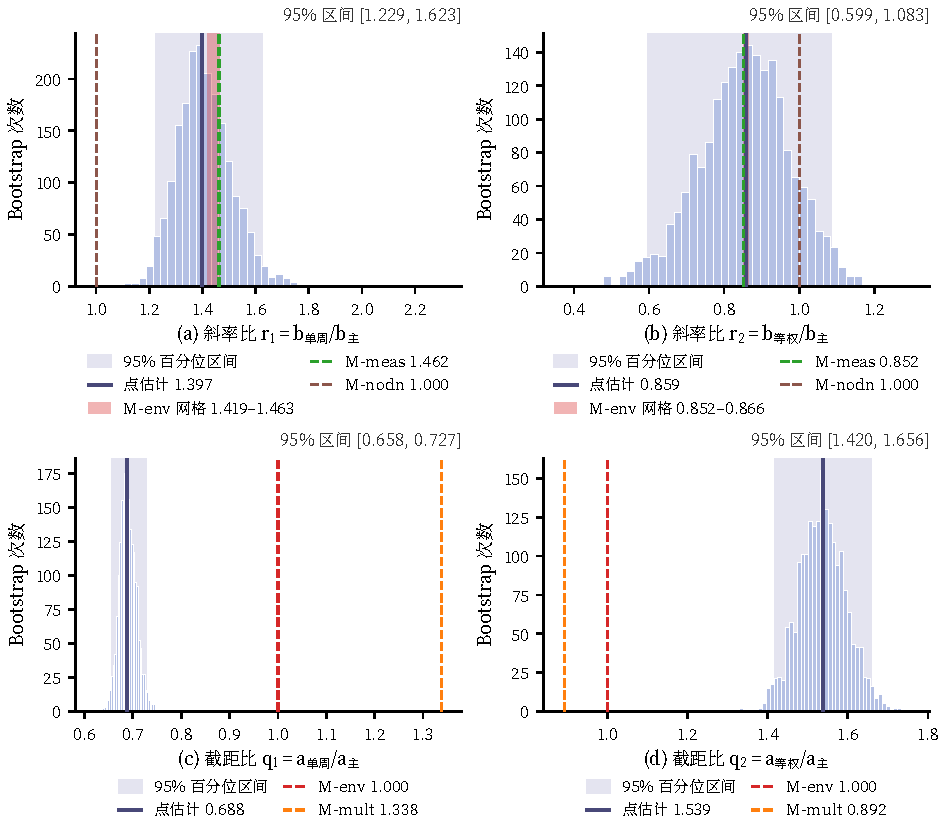
\includegraphics[width=\textwidth]{figures/fig_10_bootstrap_ratios.pdf}
  \caption{滞后权重比值的州聚类重抽分布（$N=1{,}267$ 个州周，$B=2000$，每次重估 $\overline{R}$）。(a) 斜率比 $r_1$；(b) 斜率比 $r_2$；(c) 截距比 $q_1$；(d) 截距比 $q_2$。灰色带为 95\% 百分位区间，竖线为各机制的预测（表~\ref{tab:ratios}），M-env、M-mult、M-nodn 分别为平稳环境模型、乘性报告噪声模型与分母不含计数噪声的模型。斜率比区间同时容纳平稳环境模型与纯测量误差模型，只排除 M-nodn（仅 $r_1$）；截距比区间排除平稳模型的预测，但与增长期 $\phi=0$ 的日分辨率更新过程及增长期 M-mult 的范围相交。}
  \label{fig:boot}
\end{figure}

$R_t$ 的时间相关是截距比特征的一种解释，入院延迟是另一种。$R_t$ 有时间相关时，分母越陈旧，式~\eqref{eq:mse-decomp} 中的条件偏差 $\mu_t/D_t-\Rbar$ 越大。第~\ref{sec:meth-sim}~节的一阶自回归仿真中，周间相关系数 $\phi=0.5$--0.7 时截距比为 0.64--0.76 和 1.49--1.68，与实证相符；同一每周一代的仿真在 $\phi=0$ 时为 0.86--0.94 和 1.23--1.33。以 $\mu_R=1.42$、$v_R=0.08$ 为例，$\phi=0$、0.5、0.7 时 $(q_1,q_2)$ 依次为 (0.89, 1.30)、(0.70, 1.57)、(0.64, 1.66)，斜率比 $r_1$ 都在 1.52 左右。

截距的水平只有一部分来自时间相关。在情景范围 $v_R\leq0.08$ 内，模拟截距至多为 0.058，约为独立情形理论值 $v_R/\Rbar^2$ 的 2 倍，没有一个格子的模拟截距落入实证区间。其中约 1.38 倍是归一化效应。增长期中分母滞后使 $\Rbar$ 高于 $R_t$ 自身的均值，$(1.67/1.42)^2=1.38$；在 $v_R\leq0.08$ 的六组情景中，时间相关使截距最多再乘 1.31--1.46 倍（相对同组 $\phi=0$）。要达到实证的 0.099，环境方差需取约 0.16，是情景上限的 2 倍；此时 $\mu_R=1.42$、$\phi=0.3$--0.7 的格子有 76\%--98\% 的模拟截距落入实证区间，$\mu_R=1.67$ 的对应比例只有 0--18\%。把仿真的世代块从 7 天缩短到 4 天（每周约两代）时，$a$、$q_1$、$q_2$ 的最大变化为 0.088、0.029 与 0.049；60 个格子中有 4 个同时落入实证 $a$、$q_1$、$q_2$ 的区间，其 $b/a$ 为 12.2--15.1，低于实证的 22.6（补充材料 S2.4 节）。

\subsection{报告率波动与截距}
\label{sec:res-reporting-adj}

命题~\ref{prop:report-noise}(v) 表明，只凭计数无法把截距超出的部分分给环境方差或报告波动，判别需要报告率的辅助数据。NHSN 公布的各州每周填报医院比例提供了一个可观测的代理（第~\ref{sec:meth-r3}~节）。流行初期样本中，进入比值估计量的方差 $V_\pi=0.00118$（0.00092--0.00171）；$\pi_{s,t}$ 的均值为 1.006，52\% 的州周 $\pi_{s,t}=1$，只有 5\% 的州周偏离 1 超过 0.05。三个填报制度期的 $V_\pi$ 依次为 0.0051（0.0012--0.0105）、0.119（0.083--0.177）和 0.0046（0.0036--0.0057）。自愿填报期大了两个数量级，这一期不在流行初期样本内（图~\ref{fig:reporting-adj}a）。州与州之间的填报比例差别更大，但它在比值中约去，不进入截距。

报告调整后截距几乎不变。$a=0.0991$（0.0820--0.1146），$a^*=0.0994$（0.0821--0.1150），$\Delta a=-0.0004$（$-0.0014$--0.0006），区间包含 0（图~\ref{fig:reporting-adj}b）。等价检验以 $a$ 的 5\% 为界（$\pm0.0050$），$\Delta a$ 的 90\% BCa 区间 $-0.0012$--0.0005 落在界内，可观测报告成分的贡献在这一界内与 0 等价。运行前写下的两支预测中，$-V_\pi(1+a)=-0.0013$ 落在区间内，$+0.0013$ 落在区间外，与填报比例的周间变化独立于计数、调整只增加噪声的情形相符。$\log G_t$ 对 $\log\pi_{s,t}$ 的弹性为 $-0.58$（$-1.27$--0.04），同样不支持计数随填报比例同比例变化。区间上端 0.00065 是情景超出量 $a-0.08/\Rbar^2=0.0704$ 的 0.93\%，可由填报比例观测到的报告成分不足超出量的 1\%，与填报比例无关的报告离散不受此约束。只用当周与三周等权两种权重时，$\Delta a$ 为 $+0.0005$（$-0.0001$--0.0016）与 $-0.0032$（$-0.0054$--$-0.0015$），量级都在千分之几。调整后截距比为 $q_1^*=0.680$（0.650--0.715）与 $q_2^*=1.565$（1.444--1.690）。

这一代理只记录医院是否填报，记录不到已填报医院内部的漏报，也记录不到就诊与检测行为的变化。报告率网格仿真给出了 $\Delta a$ 判据的适用范围（补充材料 S2.2 节，35 格，每格 200 次）。与填报比例无关的报告冲击的相对波动 $\tau$ 从 0 增加到 0.5 时，模拟截距从 0.10 升到 0.52，$\Delta a$ 始终接近 0。报告率随填报比例同步变化时，由于实证填报比例变化很小（中位数 0.943），判据在全部格子中的拒绝率都是 0，同步强度取到最大一档时也是如此。$\Delta a$ 因此只约束与填报比例同步的报告成分；与填报比例无关的报告波动不受上述上界约束，而截距比在增长期不能区分机制（第~\ref{sec:res-inflation}~节），这部分波动目前没有直接检验。

\begin{figure}[!tbp]
  \centering
  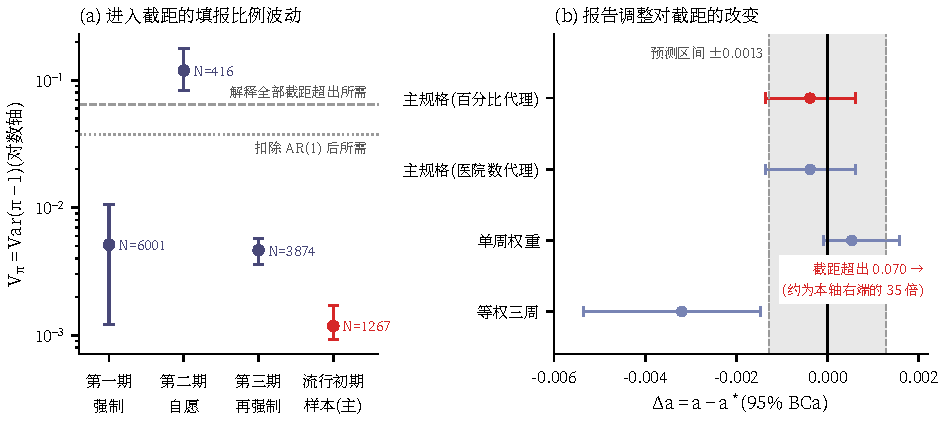
\includegraphics[width=\textwidth]{figures/fig_11_reporting_adjustment.pdf}
  \caption{报告率代理与报告调整估计量（NHSN 流感，按州聚类 $B=2000$ 次重抽）。(a) 进入截距的填报比例波动 $V_\pi=\Var(\pi_{s,t}-1)$，$\pi_{s,t}=\hat p_{s,t+1}/\sum_jw_j\hat p_{s,t-j}$，$\hat p_{s,t}$ 为填报医院比例。三个填报制度期取全面板 $D_t\geq5$ 的州周，给出百分位区间；流行初期样本（$N=1{,}267$ 个州周）为主分析，给出 BCa 区间。虚线与点线分别为把全部截距超出（$a-0.08/\overline{R}^2$）或扣除时间相关后的超出归于报告波动所需的 $V_\pi$。(b) $\Delta a=a-a^*$ 的 95\% BCa 区间，灰带为运行前写定的预测量级 $\pm V_\pi(1+a)$。}
  \label{fig:reporting-adj}
\end{figure}

\subsection{跨病原与样本外复制}
\label{sec:res-pathogens}

截距比随滞后权重变化的方向在其他病原中同样出现，但方向本身不足以区分机制。同一 NHSN 文件中，流感、COVID-19 与 RSV 的 7 个病原与窗口组合都给出 $q_1<1<q_2$，每个组合的 2,000 次重抽中同时满足两个不等式的比例都是 100\%（图~\ref{fig:pathogens}a,b）。按第~\ref{sec:meth-r3}~节的判据，7 个组合的截距比区间都与各自的增长期零假设范围相交，只有流感增长期窗口的 $q_2$（BCa 区间 1.686--2.261）位于范围上端 1.578 之外；截距比不支持任何组合的复现。

截距超出量提供主要证据（图~\ref{fig:pathogens}c）。流感的日历窗口、增长期窗口与 2025--2026 样本外季，以及 RSV 2024--2025 季窗口，截距超出量 $a-0.08/\Rbar^2$ 的 BCa 区间下端都大于 0，判为部分复现。COVID-19 的两个窗口与 RSV 增长期窗口的超出量区间包含 0 或位于 0 以下，只呈方向一致。分级结果为复现 0、部分复现 4、方向一致 3。COVID-19 在这些窗口中的 $\Rbar$ 为 1.09--1.22，不处于明显的指数增长期；情景区间按流感设定，对它的超出量只作参照。流感样本外季的截距更大，为 0.177。分级对零假设范围的取法敏感（补充材料 S2.6 节）：只用不含入院延迟的日更新格子时为复现 2、部分复现 2、方向一致 3（流感增长期窗口与 RSV 2024--2025 季窗口复现），取格点中位数或改用均值之比时为 1、3、3。主分级取包含入院延迟的全部格子，在这些取法中最保守。

报告调整在 7 个组合中的等价检验见补充材料 S2.1 节。以各组合 $a$ 的 5\% 为界，90\% BCa 区间口径下 5 个组合等价，正态近似口径下 3 个；COVID-19 增长期窗口与 RSV 增长期窗口的区间超出等价界。$\Delta a$ 区间下端大于 0 的只有流感样本外季，$\Delta a=+0.0039$（0.0017--0.0064），不到该季超出量 0.145 的 3\%，仍在该季的等价界 0.0088 以内。独立数据只提供方向参照。ILINet 门诊流感样病例监测（51 个辖区，$N=1{,}479$）给出 $q_1=0.687$（百分位区间 0.552--0.842）、$q_2=1.467$（1.406--1.531），99.7\% 的重抽满足 $q_1<1<q_2$，但病例定义不同，不参与分级。FluSurv-NET 住院监测只有 14 个站点（$N=364$），$q_1=0.686$、$q_2=1.312$，区间过宽，提供不了信息。HHS Protect 与 NHSN 在 3,417 个州周上的相关系数为 0.995，只作数据一致性核对。

\begin{figure}[!tbp]
  \centering
  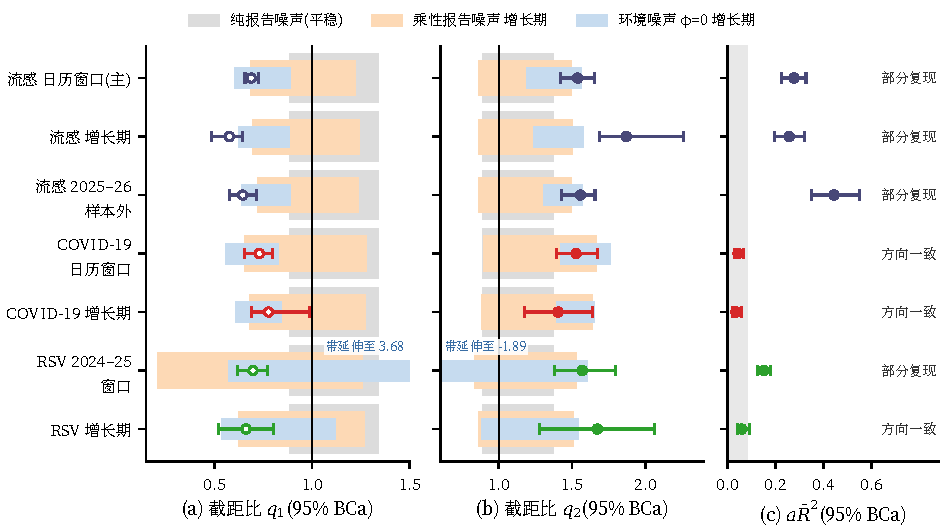
\includegraphics[width=\textwidth]{figures/fig_12_cross_pathogen.pdf}
  \caption{跨病原截距比与增长期零假设范围（NHSN 流感、COVID-19 与 RSV 的 7 个病原与窗口组合，按州聚类 $B=2000$ 次重抽的 95\% BCa 区间，各组合州周数见补充材料 S2.6 节）。(a)(b) 截距比 $q_1$（空心）与 $q_2$（实心）。灰带为平稳纯报告噪声的解析可达范围（命题~\ref{prop:report-noise}(vi)）；橙带为增长期乘性报告噪声模型（48 格）；蓝带为环境各期独立（$\phi=0$）的日分辨率更新过程（108 格，世代间隔与入院延迟各三档）。带为格点模拟平均（每格 300 次）的最小值至最大值，RSV 2024--2025 季窗口的蓝带超出坐标范围，截断并标注端点。(c) $a\overline{R}^2$，即把截距全部归于环境时隐含的 $v_R$，灰带为 $a\overline{R}^2\leq0.08$；右侧为第~\ref{sec:meth-r3}~节的分级。}
  \label{fig:pathogens}
\end{figure}

\subsection{截距的季层面成分与规模、期数}
\label{sec:res-seasons}

截距含有明显的季层面成分。三个流行季各自的截距为 0.071（0.049--0.094，$N=338$）、0.028（0.017--0.041，$N=419$）和 0.135（0.111--0.166，$N=510$），季间异质性检验 $Q=47.4$（自由度 2，$p=5\times10^{-11}$）。按增长期规则选取的 2025--2026 样本外季为 0.177（0.141--0.212，$N=663$），四季合并时 $Q=85.0$（自由度 3，$p=2.6\times10^{-18}$）。季间标准差约 0.054，约为季内抽样标准差 0.011 的 5 倍；依次去掉一季后，截距为 0.108、0.113 和 0.059（图~\ref{fig:seasons}b）。按州与按州 $\times$ 流行季聚类的区间宽度为 0.0322 与 0.0321，几乎相同。按季重抽只有 3 簇，不同的重抽组合只有 10 种，这种区间是退化的，本文没有报告。州聚类区间因此描述给定这三个流行季时的不确定性，不包含季与季之间的差别。

事先写定的规模与期数比较支持命题~\ref{prop:vR-info}。在 25 个大州中，把周计数稀疏一半使区间宽度增加 14\%，州数减半使宽度增加 46\%，满足判据，但稀疏一侧距 15\% 的阈值很近（图~\ref{fig:seasons}a）。全部 51 州的对应倍数为 0.97 与 1.48，大州组与小州组的基线宽度之比为 0.54。小州组在稀疏到四分之一时 $D_t$ 过小，拟合失稳，宽度放大到 222 倍，这对应命题~\ref{prop:vR-info} 中有限规模的 $\Omega_1/m$ 项，判据事先规定不把它作为反证。用 1、2、3 个季估计时，州聚类宽度平均为 0.042、0.038 和 0.031，加入样本外季后为 0.037，没有随季数单调变窄，原因同样是州聚类区间不包含季间方差。

两项事后分析显示，季数对截距精度的影响大于规模。把稀疏后的方差按 $1/p$ 外推到规模无穷大，全部州的重抽标准差只变为现有的 1.04 倍，大州组为 0.94 倍；规模翻倍时为 1.02 与 0.97 倍，而州数翻倍按 $\sqrt{1/2}$ 的规律为 0.71 倍。把季作为随机效应（DerSimonian--Laird 估计，$t_{S-1}$ 区间）时，三季的平均截距为 0.077（$-0.056$--0.211），区间宽 0.267，规模无穷大时仍宽 0.261；加入样本外季后（$S=4$）为 0.101（$-0.002$--0.205），宽 0.207，季间方差估计为 0.0041（Q-profile 区间 0.0012--0.0609）。第四季按增长期规则取窗，与前三季的日历窗口不同，四季结果只作敏感性参照。三季时区间跨过 0，是自由度只有 2 的结果，不能作为截距可能为负的证据。按推论~\ref{cor:season}，三季与四季的数据分别不能把季层面方差的相对标准误压到 0.82 与 0.71 以下（季均值未知时为 1.00 与 0.82），这一成分的大小因此无法由本文数据确定；大量州周决定的是给定已观测季时的精度。

\begin{figure}[!tbp]
  \centering
  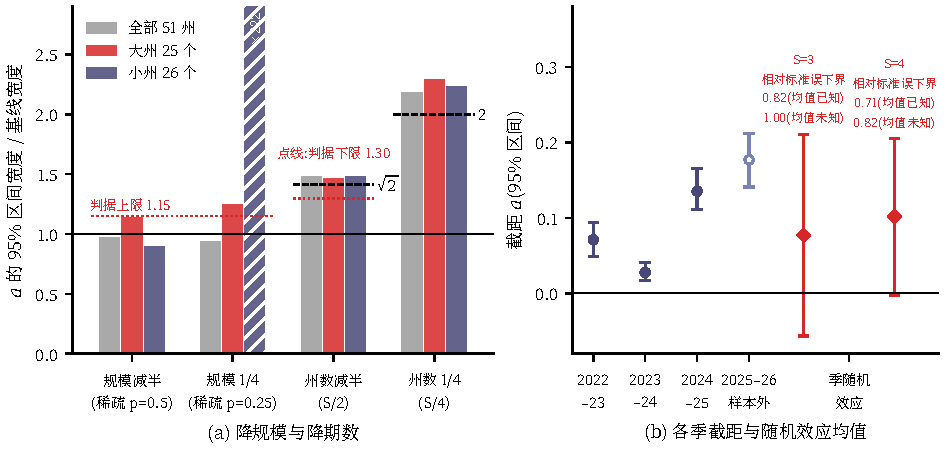
\includegraphics[width=\textwidth]{figures/fig_13_scale_vs_seasons.pdf}
  \caption{截距精度的规模与期数（NHSN 流感流行初期，$N=1{,}267$ 个州周，按州聚类 $B=2000$ 次重抽）。(a) 二项稀疏降低各州周计数、只抽部分州降低州数后，$a$ 的 95\% 百分位区间宽度相对基线的倍数；虚线为州数缩减时 $\sqrt{S/S'}$ 的预期，红色点线为事先写定的判据。小州组稀疏到四分之一时拟合失稳（222 倍，截断显示）。(b) 各季截距及州聚类 95\% 百分位区间，空心点为主分析样本之外的 2025--2026 季（增长期规则取窗）；红菱形为 DerSimonian--Laird 季随机效应的平均截距与 $t_{S-1}$ 区间（$S=3$ 与 $S=4$，事后分析），红字为推论~\ref{cor:season} 的相对标准误下界 $\sqrt{2/S}$ 与 $\sqrt{2/(S-1)}$。}
  \label{fig:seasons}
\end{figure}

\subsection{达峰期}
\label{sec:res-peak}

流行达峰后，初期基准失效。三个流行季的全国峰值周及其后 7 周共 1,220 个州周，平均增长比降到 $\Rbar_{\mathrm{peak}}=0.8075$，标准差 0.3048。继续以初期均值 1.6706 为基准时，各箱的平均损失都在 0.29--0.31，看不出随规模下降。图~\ref{fig:peak} 把这部分损失拆成基准偏移造成的常数偏差 $(\Rbar_{\mathrm{early}}-\Rbar_{\mathrm{peak}})^2/\Rbar_{\mathrm{early}}^2=0.2669$ 与箱内围绕峰期均值的波动两部分。偏差项占总损失的 88.9\%，从最小箱的 59.5\% 升到最大箱的 94.8\%。除最小箱外，峰期损失是同箱初期损失的 1.8--2.9 倍。

\begin{figure}[!tbp]
  \centering
  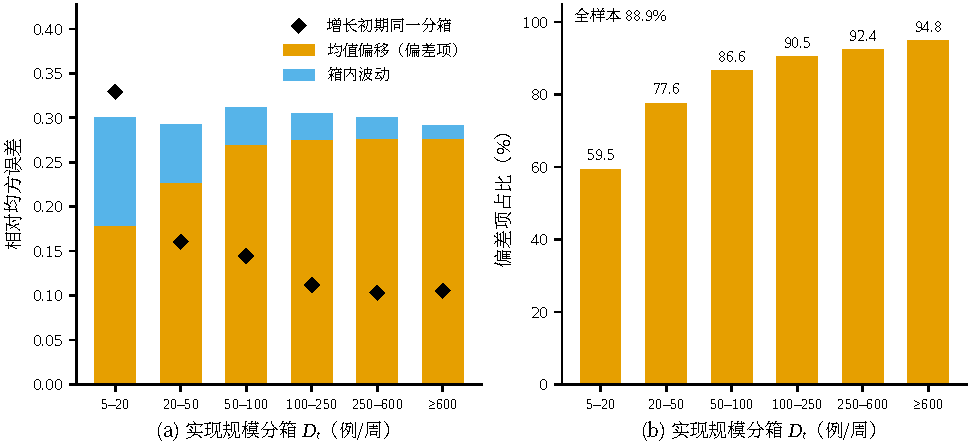
\includegraphics[width=\textwidth]{figures/fig_14_peak_decomp.pdf}
  \caption{达峰期（峰值周及其后 7 周，$N=1{,}220$ 个州周）以流行初期均值为基准时的误差分解，图中为点估计。(a) 各规模箱的平均损失，分为基准偏移造成的偏差项与箱内波动，菱形为同一分箱在流行初期的平均损失。(b) 偏差项在各箱损失中的占比。}
  \label{fig:peak}
\end{figure}

改用峰期自身均值作基准后，规模效应重新出现，$a=0.0665$（0.0467--0.0897），$b=7.927$（5.424--11.225），经验比值 119.2（64.0--225.9），平均损失 0.142。两个阶段的归一化分母不同，峰期的 $b$ 不能直接和初期的 2.243 比较。统一用 $\Rbar_{\mathrm{early}}$ 归一化后，峰期斜率为 1.852，低于初期的 2.243；不归一化时为 5.169 对 6.261。同一样本上的联合回归中，阶段交互项为 $-0.92$，95\% 区间 $-2.33$--$0.59$，包含零。达峰期规模仍然有用，现有证据不足以判断它比初期更有用或更无用。

\subsection{填报制度期与流行季}
\label{sec:res-policy}

报告制度变化提供了另一类证据。从第一期到第二期，$G_t$ 的标准差从 0.624 升到 1.823，增加 192\%，第三期回到 0.649；若填报率下降只是均匀地稀疏了病例，标准差最多放大到 $0.624\times\sqrt{91.11/54.59}=0.806$。全样本的四分位距依次为 0.638、0.594、0.652，中位绝对偏差为 0.298、0.299、0.292，看起来第二期的稳健离散度并未扩大。

这一比较受流行季构成混杂。第二期的 420 个州周中只有 55 个在流行季内，占 13\%，第一期与第三期分别为 61\% 与 58\%；而流行季内 $G_t$ 的离散度明显更大（图~\ref{fig:policy}a）。按流行季分层后，季外三期的四分位距为 0.524、0.529（0.438--0.611）和 0.448，第二期减第一期为 0.006（$-0.085$--0.090）。季内第一期为 0.710（0.667--0.749），第三期为 0.864（0.821--0.906），第二期为 1.818（1.004--2.144），第二期减第一期为 1.107（0.289--1.430）。按全面板的季内占比重新加权，第二期为 1.013（0.716--1.446），比第一期的 0.630 高 0.383（0.083--0.819）。对数增长率的四分位距给出同样的格局，季内第二期为 1.688（0.788--2.455）。

\begin{figure}[!tbp]
  \centering
  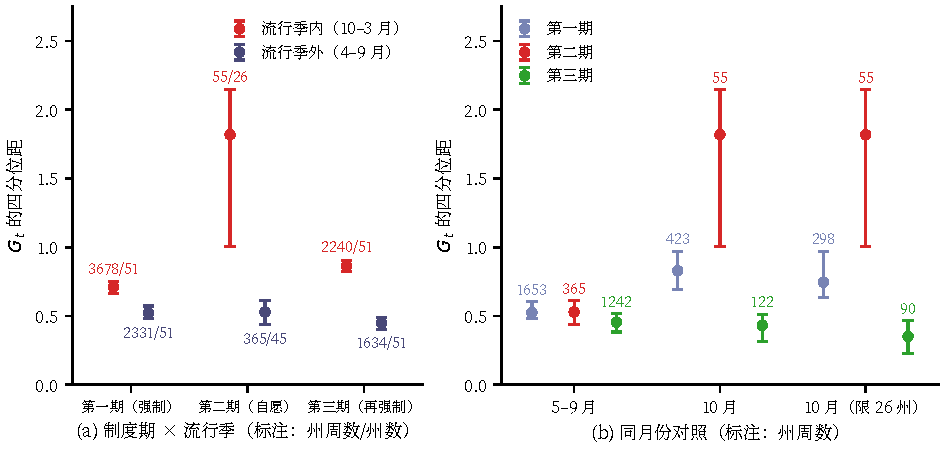
\includegraphics[width=\textwidth]{figures/fig_15_period_season_iqr.pdf}
  \caption{三个填报制度期内增长统计量 $G_t$ 的四分位距，点为估计值，误差棒为按州聚类 2,000 次重抽的 95\% 百分位区间。(a) 各期分流行季内外，标注为州周数与州数。(b) 同月份对照：5--9 月、10 月，以及只含第二期出现的 26 个州的 10 月。第二期季内的全部 55 个州周都落在 2024 年 10 月。}
  \label{fig:policy}
\end{figure}

第二期季内的证据很薄。55 个州周全部落在 2024 年 10 月，只来自 26 个州，区间宽度约为第一期的 14 倍（1.14 对 0.08）。同月份对照把季节差异与月份差异分开（图~\ref{fig:policy}b）。5--9 月第二期减第一期为 0.004（$-0.106$--0.093）；10 月为 0.988（0.139--1.364），只取这 26 个州时为 1.071（0.184--1.424）；第一期与第三期 10 月的四分位距分别为 0.829 与 0.432。以对数增长率偏离当月中位数的绝对值为因变量，分位数回归中期别 $\times$ 流行季交互在中位数处为 0.292（0.020--0.642），在 0.75 分位数处为 1.048（0.311--1.708）。剔除含缺失周的 12 个州周后，第二期季内剩 54 个州周，四分位距为 1.729（0.924--2.141），与第一期之差为 1.022（0.229--1.434）。

分层结果表明，自愿填报期的离散度扩张发生在 2024 年 10 月的流行季开端，季外几乎不变。这与填报不全的医院在病例增多时造成跳变的解释相符，也可能部分来自 2024 年 10 月本身的流行特征，现有的 26 个州、一个月的样本无法把两者分开。注~\ref{rem:reporting} 预示报告率下降会增加方差，与此只有定性联系，第二期的变化无法用 $\rho$ 的变化定量解释。

\subsection{稳健性与外部数据}
\label{sec:res-robust}

各规格下规模项都为正，经验比值在 10.6--124.7 之间变化（图~\ref{fig:forest}）。

\begin{figure}[!tbp]
  \centering
  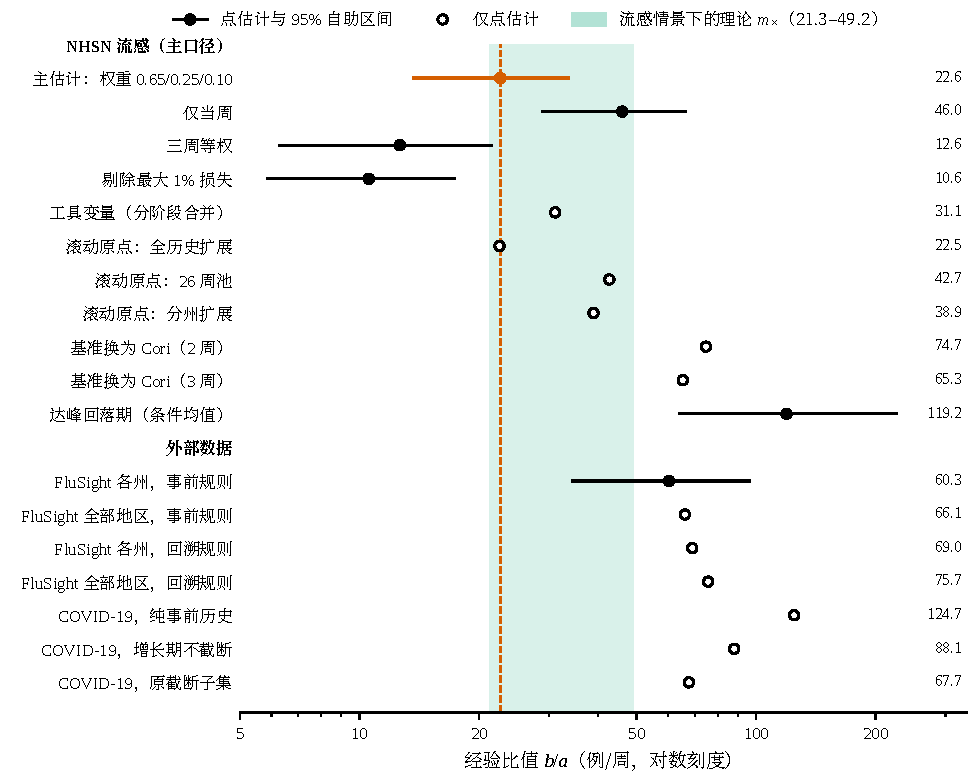
\includegraphics[width=\textwidth]{figures/fig_16_mx_forest.pdf}
  \caption{各规格下的经验比值 $b/a$。横线为原分析按州聚类重抽的 95\% 区间（只有部分规格提供；主估计行 $B=1{,}500$，故与正文 2,000 次重抽的 13.5--34.9 略有差别），阴影为理论情景区间 21.3--49.2，竖直虚线为主估计 22.6，右侧列出点估计。上部为 NHSN 数据的不同规格，下部为外部数据。}
  \label{fig:forest}
\end{figure}

$D_t$ 与 $C_{t+1}$ 同源，同期测度可能带来内生性。以滞后 3--5 周的规模作 $1/D_t$ 的工具变量，在流行季内合并样本（$N=1{,}051$）上做两阶段最小二乘\citep{wooldridge2010econometric}，得到 $b_{\mathrm{iv}}=2.53$（1.11--4.11），同一样本的普通最小二乘估计为 1.35，两者之差的 95\% 区间为 0.30--2.11，对应经验比值 31.1。第一阶段 $F$ 统计量为 1147.1，按州聚类为 312.9。$b_{\mathrm{iv}}$ 高于普通最小二乘估计，与测量误差造成的衰减偏误方向一致\citep{fuller1987measurement}。排除限制无法检验，工具变量估计只说明替代性滞后测度下规模项保持为正。

主分析的基准 $\Rbar_{\mathrm{early}}$ 用到了整个窗口的数据，属于回顾性口径。改用只含过去信息的基准后，误差整体上升。全部历史扩张窗的 $a=0.406$，$b=9.158$（5.82--12.88）；26 周滚动池的 $a=0.222$，$b=9.456$；逐州扩张窗的 $a=0.341$，$b=13.27$。三种口径下所有重抽的 $b$ 都为正，经验比值在 22.5--42.7 之间，截距在总损失中的份额为 39\%--55\%。

以 Cori 等\citep{cori2013new}的滑动窗口估计 $R_t$ 作预测，1 周、2 周与 3 周窗的平均损失为 0.436（$N=1{,}197$）、0.288（$N=1{,}244$）和 0.249（$N=1{,}251$），阶段均值基准为 0.181，直接用本周病例数预测下周的朴素方法为 0.637。三者的样本差异来自窗口内感染压力之和不足 5 的排除规则。对 Cori 基准的损失拟合式~\eqref{eq:affine}，2 周窗 $a=0.0812$、$b=6.064$，经验比值 74.7；3 周窗的经验比值为 65.3。时变估计在小规模时自身噪声较大，斜率因而更陡。

全国加总序列的流行初期平均规模约为 6,662 例/周，平均损失降到 0.0348（中位数 0.0115，$N=28$），约为单州截距的三分之一。按式~\eqref{eq:pooling}，它对应一个小于 1 的州间环境相关 $\bar c$，粗略推算约为 0.34；该推算忽略了分母噪声和 $G_t$ 的口径问题。

两组外部数据给出同样的符号。美国疾病控制与预防中心组织的 FluSight 流感住院前瞻预测中，2022--2023 季集成预测\citep{mathis2024evaluation}的评价框架见文献\citep{reich2019accuracy, cramer2022evaluation}。以集成模型事前给出的预测规模 $\widehat Y\geq5$ 筛选州级样本（$N=1{,}177$），$a=0.1295$，$b=7.805$（5.358--10.526），经验比值 60.3（34.5--95.9）；其余三种筛选口径为 66.1、69.0 和 75.7。把该集成预测在各流行阶段内的相对均方误差拆为均值偏差平方与阶段内方差，均值偏差平方在峰期（$N=206$）占 15.5\%，在上升期（$N=216$）和回落期（$N=755$）分别占 32.3\% 和 1.5\%。欧洲 11 国 2020 年 2--4 月的 COVID-19 序列\citep{flaxman2020estimating}给出更大的经验比值。纯事前口径下 $N=404$，$b=33.92$（14.60--74.99），经验比值 124.7；只取增长期为 88.1，截断子样本为 67.7。两组外部数据的经验比值都高于 NHSN 主估计，但病种、预测方法和报告系统都不同，不宜直接比较大小。
